
\documentclass[aspectratio=169,10pt]{beamer}
\usetheme{default}
\usepackage{fontspec}
\usepackage{pgfplots}
\usepackage{booktabs}
\usepackage{array}
\pgfplotsset{compat=1.18}
\usetikzlibrary{calc,positioning,backgrounds}

\setmainfont{Charter}
\setsansfont{Avenir Next}
\setmonofont{Menlo}[Scale=0.84]
\newfontfamily\dispfont{Charter}

\definecolor{ink}{HTML}{111621}
\definecolor{ink2}{HTML}{414B5E}
\definecolor{muted}{HTML}{737E93}
\definecolor{hair}{HTML}{DCE1EA}
\definecolor{hairb}{HTML}{EBEEF4}
\definecolor{sunken}{HTML}{F6F7FA}
\definecolor{cA}{HTML}{3B4E9B}
\definecolor{cB}{HTML}{00795A}
\definecolor{cC}{HTML}{B03A2E}
\definecolor{cD}{HTML}{9C5B00}
\definecolor{cN}{HTML}{8B93A3}
\definecolor{cAsoft}{HTML}{E4E8F5}
\definecolor{cBsoft}{HTML}{DDEDE7}
\definecolor{cCsoft}{HTML}{F6E3E0}

\setbeamercolor{normal text}{fg=ink2,bg=white}
\setbeamercolor{frametitle}{fg=ink,bg=white}
\setbeamercolor{structure}{fg=cA}
\setbeamerfont{frametitle}{family=\dispfont,series=\bfseries,size=\large}
\setbeamertemplate{navigation symbols}{}
\setbeamertemplate{itemize item}{\color{muted}\textbullet}
\setbeamersize{text margin left=10mm,text margin right=10mm}
\beamertemplatenavigationsymbolsempty
\AtBeginDocument{\raggedright}

% frame title: section eyebrow and rule above, title below
\makeatletter
\newcommand{\eyebrow}[1]{\def\@eyebrow{#1}}
\eyebrow{}
\setbeamertemplate{frametitle}{%
  \vskip2mm
  {\sffamily\fontsize{6.4}{7}\selectfont\color{muted}\MakeUppercase{\@eyebrow}}%
  \hfill{\ttfamily\fontsize{6.4}{7}\selectfont\color{muted}\insertframenumber\,/\,\inserttotalframenumber}\par
  \vskip0.8mm{\color{hair}\hrule height0.4pt}\vskip2.6mm
  {\usebeamerfont{frametitle}\usebeamercolor[fg]{frametitle}\insertframetitle}\par\vskip1mm}
\makeatother
\setbeamertemplate{footline}{}

% text styles
\newcommand{\lede}[1]{{\rmfamily\fontsize{10}{13.4}\selectfont\color{ink2}#1\par}}
\newcommand{\aside}[1]{{\setlength{\leftskip}{3mm}\sffamily\fontsize{7.4}{10}\selectfont
  \color{muted}\hspace*{-3mm}\rule[-0.6mm]{0.5pt}{3.4mm}\hspace{2mm}#1\par}}
\newcommand{\bodytext}[1]{{\sffamily\fontsize{7.4}{9.7}\selectfont\color{ink2}#1\par}}
\newcommand{\subhead}[1]{{\sffamily\fontsize{6.6}{9}\selectfont\bfseries\color{ink2}%
  \MakeUppercase{#1}\par\vskip0.6mm}}
\newcommand{\figcaption}[1]{{\sffamily\fontsize{6.2}{8}\selectfont\color{muted}#1\par}}
\newcommand{\str}[1]{{\color{ink}\bfseries #1}}
\newcommand{\mn}[1]{{\ttfamily #1}}
\newcommand{\rupee}{Rs\,}
\newcommand{\swatch}[1]{\tikz[baseline=-0.5mm]\fill[#1,rounded corners=0.3pt](0,0)rectangle(1.6mm,1.6mm);}
\newcommand{\legendline}[1]{{\sffamily\fontsize{6.4}{8}\selectfont\color{ink2}#1\par}}
\newcommand{\pillok}[1]{\colorbox{cBsoft}{\color{cB}\ttfamily\fontsize{6.4}{7}\selectfont #1}}
\newcommand{\pillno}[1]{\colorbox{cCsoft}{\color{cC}\ttfamily\fontsize{6.4}{7}\selectfont #1}}

% one stat in the title-slide strip
\newcommand{\statcell}[2]{%
  \begin{minipage}[t]{\dimexpr\linewidth}\raggedright
  {\dispfont\fontsize{14}{16}\selectfont\color{ink}#1}\par\vskip0.3mm
  {\sffamily\fontsize{5.8}{7}\selectfont\color{muted}\MakeUppercase{#2}}
  \end{minipage}}

\pgfplotsset{
  qrtf/.style={
    width=\plotwidth, height=\plotheight,
    axis line style={hair,line width=0.4pt},
    tick style={draw=none},
    grid=major, grid style={hairb,line width=0.4pt},
    every axis plot/.append style={line width=1.1pt},
    label style={font=\sffamily\fontsize{6.4}{8}\selectfont,color=muted},
    tick label style={font=\sffamily\fontsize{6.4}{8}\selectfont,color=muted},
    legend style={draw=none,fill=none,font=\sffamily\fontsize{6.4}{8}\selectfont,
                  text=ink2,cells={anchor=west}},
    axis x line*=bottom, axis y line*=left,
    clip=false,
  },
  nodenear/.style={
    nodes near coords, every node near coord/.append style={
      font=\ttfamily\fontsize{5.6}{7}\selectfont, color=ink2, anchor=south, yshift=0.2mm},
  },
}
\newlength{\plotwidth}\newlength{\plotheight}
\setlength{\plotwidth}{124mm}\setlength{\plotheight}{40mm}

\begin{document}

\eyebrow{QRTF Engine}
\begin{frame}[t]{A cross-sectional equity system for the NSE, and what it is worth net of costs}
\lede{Machine-learning models rank 500 Indian stocks each day; the strategy buys the best-ranked tenth and sells short the worst. Over 9.3 years the ranking has genuine predictive skill. None of the six committed configurations is profitable enough to pay for the trading it requires.}
\vskip0.8mm
\vskip2mm{\color{hair}\hrule height0.4pt}\vskip2.4mm\begin{columns}[T]\begin{column}{0.188\textwidth}\statcell{500}{names ranked daily}\end{column}\begin{column}{0.188\textwidth}\statcell{1,035}{distinct tickers}\end{column}\begin{column}{0.188\textwidth}\statcell{2,337}{trading days scored}\end{column}\begin{column}{0.188\textwidth}\statcell{9.27}{years}\end{column}\begin{column}{0.188\textwidth}\statcell{0 of 6}{configurations that clear the gate}\end{column}\end{columns}\vskip2.6mm\begin{center}\setlength{\plotwidth}{124mm}\setlength{\plotheight}{34mm}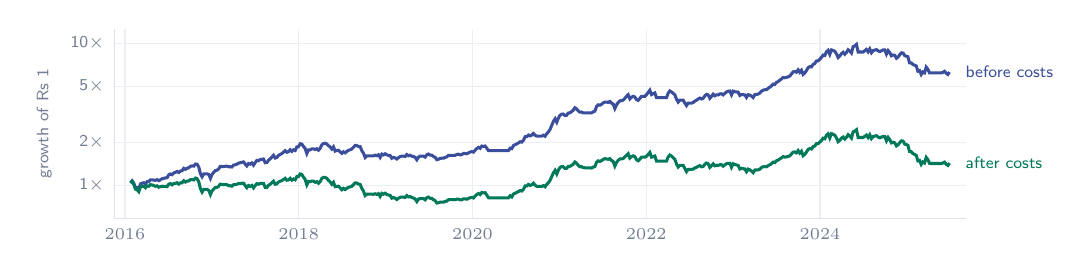
\begin{tikzpicture}\begin{axis}[qrtf,ymode=log,log basis y=10,ytick={1,2,5,10},yticklabels={1$\times$,2$\times$,5$\times$,10$\times$},xtick={2016,2018,2020,2022,2024},xticklabel style={/pgf/number format/1000 sep=},ylabel={growth of Rs 1},enlarge x limits=0.02,]\addplot[cA,line width=1.1pt,mark=none] coordinates{(2016.0630,1.04092) (2016.0822,1.07428) (2016.1014,1.03224) (2016.1205,0.96252) (2016.1397,0.96056) (2016.1589,0.93589) (2016.1781,1.02119) (2016.1973,1.03284) (2016.2164,1.04143) (2016.2356,1.02099) (2016.2548,1.05863) (2016.2740,1.06012) (2016.2932,1.09126) (2016.3123,1.09123) (2016.3315,1.08609) (2016.3507,1.08280) (2016.3699,1.09430) (2016.3890,1.07573) (2016.4082,1.09250) (2016.4274,1.11152) (2016.4466,1.11617) (2016.4658,1.12682) (2016.4849,1.12974) (2016.5041,1.18299) (2016.5233,1.20001) (2016.5425,1.18626) (2016.5616,1.22074) (2016.5808,1.23214) (2016.6000,1.25080) (2016.6192,1.22917) (2016.6384,1.25954) (2016.6575,1.26570) (2016.6767,1.31474) (2016.6959,1.29322) (2016.7151,1.31903) (2016.7342,1.32756) (2016.7534,1.36028) (2016.7726,1.36933) (2016.7918,1.36306) (2016.8110,1.41123) (2016.8301,1.40640) (2016.8493,1.34327) (2016.8685,1.20474) (2016.8877,1.14678) (2016.9068,1.20321) (2016.9260,1.20321) (2016.9452,1.20321) (2016.9644,1.19175) (2016.9836,1.11845) (2017.0000,1.18375) (2017.0192,1.22817) (2017.0384,1.26564) (2017.0575,1.27557) (2017.0767,1.30030) (2017.0959,1.35582) (2017.1151,1.35484) (2017.1342,1.35275) (2017.1534,1.36025) (2017.1726,1.36416) (2017.1918,1.34951) (2017.2110,1.34951) (2017.2301,1.34449) (2017.2493,1.38576) (2017.2685,1.39280) (2017.2877,1.40707) (2017.3068,1.43025) (2017.3260,1.44008) (2017.3452,1.44978) (2017.3644,1.46034) (2017.3836,1.40913) (2017.4027,1.36805) (2017.4219,1.42220) (2017.4411,1.40852) (2017.4603,1.43605) (2017.4795,1.38465) (2017.4986,1.44426) (2017.5178,1.49521) (2017.5370,1.48806) (2017.5562,1.51568) (2017.5753,1.52335) (2017.5945,1.53051) (2017.6137,1.44133) (2017.6329,1.44462) (2017.6521,1.50141) (2017.6712,1.53355) (2017.6904,1.57843) (2017.7096,1.62660) (2017.7288,1.55405) (2017.7479,1.57011) (2017.7671,1.62321) (2017.7863,1.64933) (2017.8055,1.67107) (2017.8247,1.71180) (2017.8438,1.75342) (2017.8630,1.70850) (2017.8822,1.72496) (2017.9014,1.77880) (2017.9205,1.73382) (2017.9397,1.77566) (2017.9589,1.75666) (2017.9781,1.86335) (2017.9973,1.86801) (2018.0164,1.96157) (2018.0356,1.95017) (2018.0548,1.87672) (2018.0740,1.81656) (2018.0932,1.67402) (2018.1123,1.77681) (2018.1315,1.77681) (2018.1507,1.80756) (2018.1699,1.80756) (2018.1890,1.78538) (2018.2082,1.80824) (2018.2274,1.76684) (2018.2466,1.81981) (2018.2658,1.92852) (2018.2849,1.96900) (2018.3041,1.97814) (2018.3233,1.95458) (2018.3425,1.89794) (2018.3616,1.86303) (2018.3808,1.79985) (2018.4000,1.86371) (2018.4192,1.74090) (2018.4384,1.75685) (2018.4575,1.76397) (2018.4767,1.72021) (2018.4959,1.67789) (2018.5151,1.72146) (2018.5342,1.69210) (2018.5534,1.73141) (2018.5726,1.76334) (2018.5918,1.77915) (2018.6110,1.80031) (2018.6301,1.85071) (2018.6493,1.90855) (2018.6685,1.90477) (2018.6877,1.87447) (2018.7068,1.86985) (2018.7260,1.75379) (2018.7452,1.68345) (2018.7644,1.56849) (2018.7836,1.60951) (2018.8027,1.60951) (2018.8219,1.60951) (2018.8411,1.60951) (2018.8603,1.61132) (2018.8795,1.63019) (2018.8986,1.61536) (2018.9178,1.63939) (2018.9370,1.57153) (2018.9562,1.65772) (2018.9753,1.63685) (2018.9945,1.66600) (2019.0137,1.63919) (2019.0329,1.62140) (2019.0521,1.61813) (2019.0712,1.54918) (2019.0904,1.57210) (2019.1096,1.55748) (2019.1288,1.52990) (2019.1479,1.56568) (2019.1671,1.59004) (2019.1863,1.60313) (2019.2055,1.60375) (2019.2247,1.59417) (2019.2438,1.64590) (2019.2630,1.61388) (2019.2822,1.62663) (2019.3014,1.60159) (2019.3205,1.59582) (2019.3397,1.57385) (2019.3589,1.51166) (2019.3781,1.57811) (2019.3973,1.60247) (2019.4164,1.60247) (2019.4356,1.60247) (2019.4548,1.57872) (2019.4740,1.64004) (2019.4932,1.65971) (2019.5123,1.62853) (2019.5315,1.63011) (2019.5507,1.59375) (2019.5699,1.57572) (2019.5890,1.51469) (2019.6082,1.52619) (2019.6274,1.54294) (2019.6466,1.55206) (2019.6658,1.55042) (2019.6849,1.57220) (2019.7041,1.58272) (2019.7233,1.62622) (2019.7425,1.62622) (2019.7616,1.62622) (2019.7808,1.62622) (2019.8000,1.62622) (2019.8192,1.64868) (2019.8384,1.65441) (2019.8575,1.63631) (2019.8767,1.64484) (2019.8959,1.67386) (2019.9151,1.67569) (2019.9342,1.66654) (2019.9534,1.69132) (2019.9726,1.71389) (2019.9918,1.72724) (2020.0110,1.71168) (2020.0301,1.76609) (2020.0493,1.81597) (2020.0685,1.84931) (2020.0877,1.82034) (2020.1068,1.89021) (2020.1260,1.87841) (2020.1452,1.89050) (2020.1644,1.82435) (2020.1836,1.75213) (2020.2027,1.75213) (2020.2219,1.75213) (2020.2411,1.75213) (2020.2603,1.75213) (2020.2795,1.75213) (2020.2986,1.75213) (2020.3178,1.75213) (2020.3370,1.75213) (2020.3562,1.75213) (2020.3753,1.75213) (2020.3945,1.75213) (2020.4137,1.75213) (2020.4329,1.82294) (2020.4521,1.80983) (2020.4712,1.90365) (2020.4904,1.92979) (2020.5096,1.95936) (2020.5288,1.98850) (2020.5479,2.02551) (2020.5671,2.01380) (2020.5863,2.07473) (2020.6055,2.19816) (2020.6247,2.20127) (2020.6438,2.26106) (2020.6630,2.22808) (2020.6822,2.25835) (2020.7014,2.31886) (2020.7205,2.25148) (2020.7397,2.21911) (2020.7589,2.21911) (2020.7781,2.21911) (2020.7973,2.21911) (2020.8164,2.25470) (2020.8356,2.21702) (2020.8548,2.31071) (2020.8740,2.37955) (2020.8932,2.48135) (2020.9123,2.64585) (2020.9315,2.82318) (2020.9507,2.94268) (2020.9699,2.78421) (2020.9890,2.97837) (2021.0055,3.10727) (2021.0247,3.17038) (2021.0438,3.17789) (2021.0630,3.10658) (2021.0822,3.11362) (2021.1014,3.22830) (2021.1205,3.24407) (2021.1397,3.30210) (2021.1589,3.38211) (2021.1781,3.51781) (2021.1973,3.45721) (2021.2164,3.34739) (2021.2356,3.27705) (2021.2548,3.28459) (2021.2740,3.24127) (2021.2932,3.24127) (2021.3123,3.24127) (2021.3315,3.24127) (2021.3507,3.24127) (2021.3699,3.23407) (2021.3890,3.29354) (2021.4082,3.32907) (2021.4274,3.58700) (2021.4466,3.69259) (2021.4658,3.67014) (2021.4849,3.72279) (2021.5041,3.80992) (2021.5233,3.86243) (2021.5425,3.85665) (2021.5616,3.84422) (2021.5808,3.89729) (2021.6000,3.79295) (2021.6192,3.74077) (2021.6384,3.47752) (2021.6575,3.69287) (2021.6767,3.83472) (2021.6959,3.93946) (2021.7151,3.94938) (2021.7342,3.98768) (2021.7534,4.10180) (2021.7726,4.23576) (2021.7918,4.35097) (2021.8110,4.06681) (2021.8301,4.17563) (2021.8493,4.24003) (2021.8685,4.19262) (2021.8877,4.01547) (2021.9068,3.96841) (2021.9260,4.09488) (2021.9452,4.24084) (2021.9644,4.24084) (2021.9836,4.24084) (2022.0027,4.35692) (2022.0219,4.50837) (2022.0411,4.68113) (2022.0603,4.36074) (2022.0795,4.42469) (2022.0986,4.48119) (2022.1178,4.14787) (2022.1370,4.14787) (2022.1562,4.14787) (2022.1753,4.14787) (2022.1945,4.14787) (2022.2137,4.14787) (2022.2329,4.14787) (2022.2521,4.45896) (2022.2712,4.62705) (2022.2904,4.55299) (2022.3096,4.44917) (2022.3288,4.34622) (2022.3479,4.04357) (2022.3671,3.85915) (2022.3863,3.98215) (2022.4055,3.98215) (2022.4247,3.98215) (2022.4438,3.80043) (2022.4630,3.64814) (2022.4822,3.79446) (2022.5014,3.79446) (2022.5205,3.79446) (2022.5397,3.83583) (2022.5589,3.92227) (2022.5781,3.97555) (2022.5973,4.06394) (2022.6164,4.12190) (2022.6356,4.05855) (2022.6548,4.10520) (2022.6740,4.26785) (2022.6932,4.37205) (2022.7123,4.33888) (2022.7315,4.10733) (2022.7507,4.23287) (2022.7699,4.38835) (2022.7890,4.27448) (2022.8082,4.34459) (2022.8274,4.33362) (2022.8466,4.40749) (2022.8658,4.41872) (2022.8849,4.33960) (2022.9041,4.44661) (2022.9233,4.55152) (2022.9425,4.60382) (2022.9616,4.62123) (2022.9808,4.34398) (2023.0000,4.61214) (2023.0192,4.56672) (2023.0384,4.55376) (2023.0575,4.53387) (2023.0767,4.29656) (2023.0959,4.36100) (2023.1151,4.34868) (2023.1342,4.34450) (2023.1534,4.16301) (2023.1726,4.35228) (2023.1918,4.32177) (2023.2110,4.25258) (2023.2301,4.15652) (2023.2493,4.35597) (2023.2685,4.37143) (2023.2877,4.39374) (2023.3068,4.46476) (2023.3260,4.61345) (2023.3452,4.67875) (2023.3644,4.71811) (2023.3836,4.72059) (2023.4027,4.82509) (2023.4219,4.92553) (2023.4411,5.02000) (2023.4603,5.17455) (2023.4795,5.14679) (2023.4986,5.31660) (2023.5178,5.39092) (2023.5370,5.51254) (2023.5562,5.62390) (2023.5753,5.75488) (2023.5945,5.72979) (2023.6137,5.76234) (2023.6329,5.82302) (2023.6521,5.89252) (2023.6712,6.10202) (2023.6904,6.30574) (2023.7096,6.34472) (2023.7288,6.26972) (2023.7479,6.51911) (2023.7671,6.26472) (2023.7863,6.47610) (2023.8055,6.05176) (2023.8247,6.20169) (2023.8438,6.45502) (2023.8630,6.74623) (2023.8822,6.87106) (2023.9014,6.83800) (2023.9205,7.12699) (2023.9397,7.21828) (2023.9589,7.52708) (2023.9781,7.55022) (2023.9973,7.76088) (2024.0164,7.97850) (2024.0356,8.29045) (2024.0548,8.24468) (2024.0740,8.74168) (2024.0932,8.95019) (2024.1123,8.38502) (2024.1315,9.00796) (2024.1507,8.93173) (2024.1699,8.80656) (2024.1890,8.44601) (2024.2082,7.96405) (2024.2274,8.16623) (2024.2466,8.47904) (2024.2658,8.66943) (2024.2849,8.39808) (2024.3041,8.64594) (2024.3233,9.03715) (2024.3425,8.83750) (2024.3616,8.57286) (2024.3808,9.50270) (2024.4000,9.62734) (2024.4192,9.85902) (2024.4384,8.70779) (2024.4575,8.70779) (2024.4767,8.70779) (2024.4959,8.70779) (2024.5151,8.89850) (2024.5342,9.08284) (2024.5534,8.73541) (2024.5726,9.15397) (2024.5918,8.60854) (2024.6110,8.90759) (2024.6301,8.97877) (2024.6493,9.06097) (2024.6685,8.87129) (2024.6877,8.77687) (2024.7068,8.88616) (2024.7260,9.01429) (2024.7452,9.01412) (2024.7644,8.41727) (2024.7836,8.91485) (2024.8027,8.62011) (2024.8219,8.18829) (2024.8411,8.29688) (2024.8603,8.24755) (2024.8795,7.86471) (2024.8986,8.03029) (2024.9178,8.33745) (2024.9370,8.59921) (2024.9562,8.56640) (2024.9753,8.18909) (2024.9945,8.14110) (2025.0110,8.07234) (2025.0301,7.30058) (2025.0493,7.30058) (2025.0685,7.11310) (2025.0877,7.02777) (2025.1068,6.95231) (2025.1260,6.37459) (2025.1452,6.44190) (2025.1644,6.04590) (2025.1836,6.29508) (2025.2027,6.20721) (2025.2219,6.81169) (2025.2411,6.58645) (2025.2603,6.19814) (2025.2795,6.19814) (2025.2986,6.19814) (2025.3178,6.19814) (2025.3370,6.19814) (2025.3562,6.19814) (2025.3753,6.19814) (2025.3945,6.19814) (2025.4137,6.25530) (2025.4329,6.36143) (2025.4521,6.16398) (2025.4712,6.04971) (2025.4904,6.28794)};\node[anchor=west,font=\sffamily\fontsize{6.4}{8}\selectfont,text=cA,xshift=0.8mm] at (axis cs:2025.4904,6.28794){before costs};\addplot[cB,line width=1.1pt,mark=none] coordinates{(2016.0630,1.03513) (2016.0822,1.06260) (2016.1014,1.01232) (2016.1205,0.93725) (2016.1397,0.92956) (2016.1589,0.90023) (2016.1781,0.97320) (2016.1973,0.98041) (2016.2164,0.98228) (2016.2356,0.95964) (2016.2548,0.98861) (2016.2740,0.98339) (2016.2932,1.00929) (2016.3123,1.00485) (2016.3315,0.99295) (2016.3507,0.98352) (2016.3699,0.98917) (2016.3890,0.96790) (2016.4082,0.97691) (2016.4274,0.98351) (2016.4466,0.98007) (2016.4658,0.98242) (2016.4849,0.97763) (2016.5041,1.01671) (2016.5233,1.02638) (2016.5425,1.00569) (2016.5616,1.02777) (2016.5808,1.03044) (2016.6000,1.04093) (2016.6192,1.01862) (2016.6384,1.04019) (2016.6575,1.04060) (2016.6767,1.07498) (2016.6959,1.05233) (2016.7151,1.06908) (2016.7342,1.07204) (2016.7534,1.09373) (2016.7726,1.09660) (2016.7918,1.08980) (2016.8110,1.12288) (2016.8301,1.11200) (2016.8493,1.05768) (2016.8685,0.94498) (2016.8877,0.89425) (2016.9068,0.93444) (2016.9260,0.93444) (2016.9452,0.93444) (2016.9644,0.91908) (2016.9836,0.85838) (2017.0000,0.90615) (2017.0192,0.93616) (2017.0384,0.96126) (2017.0575,0.96478) (2017.0767,0.97999) (2017.0959,1.01753) (2017.1151,1.01396) (2017.1342,1.00765) (2017.1534,1.00945) (2017.1726,1.00863) (2017.1918,0.99358) (2017.2110,0.99091) (2017.2301,0.98343) (2017.2493,1.00863) (2017.2685,1.00911) (2017.2877,1.01622) (2017.3068,1.02698) (2017.3260,1.02921) (2017.3452,1.03139) (2017.3644,1.03444) (2017.3836,0.99464) (2017.4027,0.96046) (2017.4219,0.99447) (2017.4411,0.98058) (2017.4603,0.99636) (2017.4795,0.95703) (2017.4986,0.99441) (2017.5178,1.02561) (2017.5370,1.01610) (2017.5562,1.03009) (2017.5753,1.03093) (2017.5945,1.02920) (2017.6137,0.96521) (2017.6329,0.96403) (2017.6521,0.99887) (2017.6712,1.01539) (2017.6904,1.04045) (2017.7096,1.06761) (2017.7288,1.01571) (2017.7479,1.02190) (2017.7671,1.05402) (2017.7863,1.06746) (2017.8055,1.07784) (2017.8247,1.09837) (2017.8438,1.11814) (2017.8630,1.08415) (2017.8822,1.08931) (2017.9014,1.11856) (2017.9205,1.08522) (2017.9397,1.10634) (2017.9589,1.09075) (2017.9781,1.15223) (2017.9973,1.15094) (2018.0164,1.20107) (2018.0356,1.18951) (2018.0548,1.13932) (2018.0740,1.09961) (2018.0932,1.00628) (2018.1123,1.06228) (2018.1315,1.05911) (2018.1507,1.06983) (2018.1699,1.06690) (2018.1890,1.04884) (2018.2082,1.05835) (2018.2274,1.03148) (2018.2466,1.06058) (2018.2658,1.11811) (2018.2849,1.13584) (2018.3041,1.13602) (2018.3233,1.11703) (2018.3425,1.08085) (2018.3616,1.05504) (2018.3808,1.01552) (2018.4000,1.04844) (2018.4192,0.97588) (2018.4384,0.98176) (2018.4575,0.98289) (2018.4767,0.95599) (2018.4959,0.92945) (2018.5151,0.95060) (2018.5342,0.93193) (2018.5534,0.95149) (2018.5726,0.96675) (2018.5918,0.97320) (2018.6110,0.98242) (2018.6301,1.00871) (2018.6493,1.03893) (2018.6685,1.03582) (2018.6877,1.01778) (2018.7068,1.01375) (2018.7260,0.94930) (2018.7452,0.90849) (2018.7644,0.84499) (2018.7836,0.86407) (2018.8027,0.86407) (2018.8219,0.86407) (2018.8411,0.86407) (2018.8603,0.86265) (2018.8795,0.86989) (2018.8986,0.86100) (2018.9178,0.87207) (2018.9370,0.83289) (2018.9562,0.87614) (2018.9753,0.86363) (2018.9945,0.87760) (2019.0137,0.86187) (2019.0329,0.85131) (2019.0521,0.84753) (2019.0712,0.80945) (2019.0904,0.81915) (2019.1096,0.80906) (2019.1288,0.79235) (2019.1479,0.80975) (2019.1671,0.82063) (2019.1863,0.82547) (2019.2055,0.82463) (2019.2247,0.81930) (2019.2438,0.84463) (2019.2630,0.82635) (2019.2822,0.83167) (2019.3014,0.81805) (2019.3205,0.81243) (2019.3397,0.79966) (2019.3589,0.76668) (2019.3781,0.79826) (2019.3973,0.80480) (2019.4164,0.80480) (2019.4356,0.80480) (2019.4548,0.78877) (2019.4740,0.81614) (2019.4932,0.82466) (2019.5123,0.80839) (2019.5315,0.80748) (2019.5507,0.78890) (2019.5699,0.77896) (2019.5890,0.74808) (2019.6082,0.75220) (2019.6274,0.75907) (2019.6466,0.76084) (2019.6658,0.75890) (2019.6849,0.76850) (2019.7041,0.77223) (2019.7233,0.78997) (2019.7425,0.78997) (2019.7616,0.78997) (2019.7808,0.78997) (2019.8000,0.78997) (2019.8192,0.79719) (2019.8384,0.79801) (2019.8575,0.78714) (2019.8767,0.78920) (2019.8959,0.80171) (2019.9151,0.80129) (2019.9342,0.79604) (2019.9534,0.80664) (2019.9726,0.81549) (2019.9918,0.82087) (2020.0110,0.81233) (2020.0301,0.83751) (2020.0493,0.86002) (2020.0685,0.87440) (2020.0877,0.85871) (2020.1068,0.88879) (2020.1260,0.88211) (2020.1452,0.88587) (2020.1644,0.85220) (2020.1836,0.81537) (2020.2027,0.81349) (2020.2219,0.81349) (2020.2411,0.81349) (2020.2603,0.81349) (2020.2795,0.81349) (2020.2986,0.81349) (2020.3178,0.81349) (2020.3370,0.81349) (2020.3562,0.81349) (2020.3753,0.81349) (2020.3945,0.81349) (2020.4137,0.81349) (2020.4329,0.84163) (2020.4521,0.82597) (2020.4712,0.86691) (2020.4904,0.87708) (2020.5096,0.88970) (2020.5288,0.90125) (2020.5479,0.91638) (2020.5671,0.90930) (2020.5863,0.93507) (2020.6055,0.98838) (2020.6247,0.98731) (2020.6438,1.01288) (2020.6630,0.99586) (2020.6822,1.00755) (2020.7014,1.03263) (2020.7205,0.99932) (2020.7397,0.98205) (2020.7589,0.98205) (2020.7781,0.98205) (2020.7973,0.98205) (2020.8164,0.99320) (2020.8356,0.97493) (2020.8548,1.01413) (2020.8740,1.04179) (2020.8932,1.08397) (2020.9123,1.15060) (2020.9315,1.22436) (2020.9507,1.27257) (2020.9699,1.19977) (2020.9890,1.27925) (2021.0055,1.33034) (2021.0247,1.35327) (2021.0438,1.35037) (2021.0630,1.31312) (2021.0822,1.31269) (2021.1014,1.35690) (2021.1205,1.35895) (2021.1397,1.37779) (2021.1589,1.40567) (2021.1781,1.45822) (2021.1973,1.43000) (2021.2164,1.38237) (2021.2356,1.34966) (2021.2548,1.35127) (2021.2740,1.33095) (2021.2932,1.32722) (2021.3123,1.32722) (2021.3315,1.32722) (2021.3507,1.32722) (2021.3699,1.32056) (2021.3890,1.34167) (2021.4082,1.35328) (2021.4274,1.44954) (2021.4466,1.48533) (2021.4658,1.47146) (2021.4849,1.48934) (2021.5041,1.52155) (2021.5233,1.53922) (2021.5425,1.53188) (2021.5616,1.52265) (2021.5808,1.54025) (2021.6000,1.49377) (2021.6192,1.47047) (2021.6384,1.36578) (2021.6575,1.44780) (2021.6767,1.49755) (2021.6959,1.53429) (2021.7151,1.53224) (2021.7342,1.54335) (2021.7534,1.58343) (2021.7726,1.62932) (2021.7918,1.66917) (2021.8110,1.55466) (2021.8301,1.59118) (2021.8493,1.61205) (2021.8685,1.59004) (2021.8877,1.51548) (2021.9068,1.48854) (2021.9260,1.52763) (2021.9452,1.57586) (2021.9644,1.57586) (2021.9836,1.57586) (2022.0027,1.60270) (2022.0219,1.64772) (2022.0411,1.70361) (2022.0603,1.57723) (2022.0795,1.59413) (2022.0986,1.60674) (2022.1178,1.48031) (2022.1370,1.47697) (2022.1562,1.47697) (2022.1753,1.47697) (2022.1945,1.47697) (2022.2137,1.47697) (2022.2329,1.47697) (2022.2521,1.58119) (2022.2712,1.63431) (2022.2904,1.60516) (2022.3096,1.56371) (2022.3288,1.52204) (2022.3479,1.41199) (2022.3671,1.34213) (2022.3863,1.38104) (2022.4055,1.38104) (2022.4247,1.38104) (2022.4438,1.31289) (2022.4630,1.24765) (2022.4822,1.29313) (2022.5014,1.29313) (2022.5205,1.29313) (2022.5397,1.29952) (2022.5589,1.32427) (2022.5781,1.33629) (2022.5973,1.36023) (2022.6164,1.37390) (2022.6356,1.34761) (2022.6548,1.35610) (2022.6740,1.40519) (2022.6932,1.43433) (2022.7123,1.41755) (2022.7315,1.33566) (2022.7507,1.36966) (2022.7699,1.41449) (2022.7890,1.37062) (2022.8082,1.38546) (2022.8274,1.37755) (2022.8466,1.39404) (2022.8658,1.39397) (2022.8849,1.36356) (2022.9041,1.39216) (2022.9233,1.41779) (2022.9425,1.42595) (2022.9616,1.42759) (2022.9808,1.33784) (2023.0000,1.41638) (2023.0192,1.39822) (2023.0384,1.39036) (2023.0575,1.37914) (2023.0767,1.30114) (2023.0959,1.31554) (2023.1151,1.30836) (2023.1342,1.30290) (2023.1534,1.24583) (2023.1726,1.29882) (2023.1918,1.28399) (2023.2110,1.25815) (2023.2301,1.22601) (2023.2493,1.27992) (2023.2685,1.28086) (2023.2877,1.28240) (2023.3068,1.29652) (2023.3260,1.33393) (2023.3452,1.34749) (2023.3644,1.35368) (2023.3836,1.34852) (2023.4027,1.37355) (2023.4219,1.39564) (2023.4411,1.41638) (2023.4603,1.45631) (2023.4795,1.44430) (2023.4986,1.48846) (2023.5178,1.50370) (2023.5370,1.53433) (2023.5562,1.55965) (2023.5753,1.59108) (2023.5945,1.57885) (2023.6137,1.58388) (2023.6329,1.59649) (2023.6521,1.61097) (2023.6712,1.66294) (2023.6904,1.71160) (2023.7096,1.71726) (2023.7288,1.69197) (2023.7479,1.75474) (2023.7671,1.68339) (2023.7863,1.73606) (2023.8055,1.61631) (2023.8247,1.65180) (2023.8438,1.71462) (2023.8630,1.78723) (2023.8822,1.81580) (2023.9014,1.80095) (2023.9205,1.87239) (2023.9397,1.89014) (2023.9589,1.96415) (2023.9781,1.96533) (2023.9973,2.01618) (2024.0164,2.06870) (2024.0356,2.14700) (2024.0548,2.12906) (2024.0740,2.25480) (2024.0932,2.30364) (2024.1123,2.15401) (2024.1315,2.31181) (2024.1507,2.28860) (2024.1699,2.25200) (2024.1890,2.15689) (2024.2082,2.02880) (2024.2274,2.07393) (2024.2466,2.14937) (2024.2658,2.18827) (2024.2849,2.11743) (2024.3041,2.17742) (2024.3233,2.27325) (2024.3425,2.22055) (2024.3616,2.15098) (2024.3808,2.38027) (2024.4000,2.40880) (2024.4192,2.46242) (2024.4384,2.17033) (2024.4575,2.17033) (2024.4767,2.17033) (2024.4959,2.17033) (2024.5151,2.21306) (2024.5342,2.25685) (2024.5534,2.16871) (2024.5726,2.26997) (2024.5918,2.13256) (2024.6110,2.20451) (2024.6301,2.22038) (2024.6493,2.23687) (2024.6685,2.18616) (2024.6877,2.16008) (2024.7068,2.18388) (2024.7260,2.20986) (2024.7452,2.20520) (2024.7644,2.05691) (2024.7836,2.17451) (2024.8027,2.09925) (2024.8219,1.98967) (2024.8411,2.00911) (2024.8603,1.99051) (2024.8795,1.89397) (2024.8986,1.92972) (2024.9178,1.99828) (2024.9370,2.05693) (2024.9562,2.04549) (2024.9753,1.94880) (2024.9945,1.93505) (2025.0110,1.91352) (2025.0301,1.72845) (2025.0493,1.72487) (2025.0685,1.67361) (2025.0877,1.65019) (2025.1068,1.62441) (2025.1260,1.48564) (2025.1452,1.49737) (2025.1644,1.40206) (2025.1836,1.45808) (2025.2027,1.43612) (2025.2219,1.57068) (2025.2411,1.51679) (2025.2603,1.42517) (2025.2795,1.42250) (2025.2986,1.42250) (2025.3178,1.42250) (2025.3370,1.42250) (2025.3562,1.42250) (2025.3753,1.42250) (2025.3945,1.42250) (2025.4137,1.43216) (2025.4329,1.45433) (2025.4521,1.40687) (2025.4712,1.37878) (2025.4904,1.43165)};\node[anchor=west,font=\sffamily\fontsize{6.4}{8}\selectfont,text=cB,xshift=0.8mm] at (axis cs:2025.4904,1.43165){after costs};\end{axis}\end{tikzpicture}\end{center}\figcaption{Growth of \rupee{}1 in the best of the six configurations (long only, 21-day target), before and after measured transaction costs. Log scale. 2016-01-21 to 2025-06-27.}
\note{Open on the gap. Everything in the deck is an account of where that gap comes from and why it cannot be closed. The skill is real; the cost of harvesting it is larger.}\end{frame}
\eyebrow{The system}
\begin{frame}[t]{Ranking, not forecasting}
\begin{columns}[T]\begin{column}{0.40\textwidth}\bodytext{The system does not try to predict whether the market will rise or fall. Each trading day it ranks all 500 stocks against one another by predicted return over the next few days.}
\vskip0.8mm
\bodytext{It then buys the top 10\% and \emph{sells short} the bottom 10\% — short selling means borrowing a share, selling it, and buying it back later, which profits when the price falls.}
\vskip0.8mm
\bodytext{Because the strategy is long and short at the same time, a general market move affects both sides and largely cancels. What is left depends on whether the \emph{ordering} was right.}\end{column}\begin{column}{0.575\textwidth}\begin{center}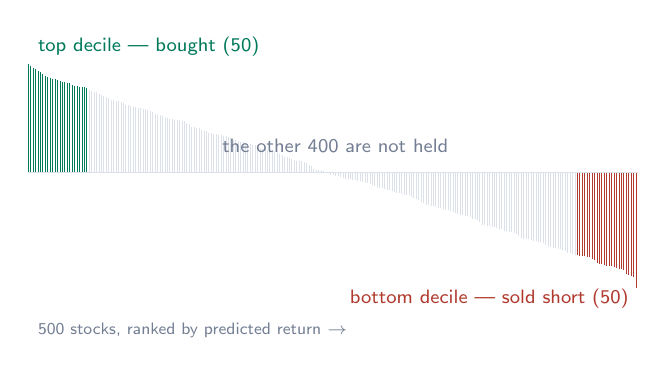
\begin{tikzpicture}[x=1mm,y=1mm]\draw[cB,line width=0.3pt](0.00,0)--(0.00,13.761);\draw[cB,line width=0.3pt](0.31,0)--(0.31,13.525);\draw[cB,line width=0.3pt](0.62,0)--(0.62,13.336);\draw[cB,line width=0.3pt](0.93,0)--(0.93,13.185);\draw[cB,line width=0.3pt](1.24,0)--(1.24,12.919);\draw[cB,line width=0.3pt](1.55,0)--(1.55,12.726);\draw[cB,line width=0.3pt](1.86,0)--(1.86,12.526);\draw[cB,line width=0.3pt](2.17,0)--(2.17,12.327);\draw[cB,line width=0.3pt](2.48,0)--(2.48,12.164);\draw[cB,line width=0.3pt](2.79,0)--(2.79,11.949);\draw[cB,line width=0.3pt](3.10,0)--(3.10,11.934);\draw[cB,line width=0.3pt](3.41,0)--(3.41,11.829);\draw[cB,line width=0.3pt](3.72,0)--(3.72,11.699);\draw[cB,line width=0.3pt](4.03,0)--(4.03,11.641);\draw[cB,line width=0.3pt](4.34,0)--(4.34,11.488);\draw[cB,line width=0.3pt](4.65,0)--(4.65,11.453);\draw[cB,line width=0.3pt](4.96,0)--(4.96,11.381);\draw[cB,line width=0.3pt](5.27,0)--(5.27,11.332);\draw[cB,line width=0.3pt](5.58,0)--(5.58,11.179);\draw[cB,line width=0.3pt](5.89,0)--(5.89,11.013);\draw[cB,line width=0.3pt](6.20,0)--(6.20,10.986);\draw[cB,line width=0.3pt](6.51,0)--(6.51,10.889);\draw[cB,line width=0.3pt](6.82,0)--(6.82,10.869);\draw[cB,line width=0.3pt](7.13,0)--(7.13,10.821);\draw[cB,line width=0.3pt](7.44,0)--(7.44,10.677);\draw[hair,line width=0.3pt](7.75,0)--(7.75,10.487);\draw[hair,line width=0.3pt](8.06,0)--(8.06,10.359);\draw[hair,line width=0.3pt](8.37,0)--(8.37,10.289);\draw[hair,line width=0.3pt](8.68,0)--(8.68,10.216);\draw[hair,line width=0.3pt](8.99,0)--(8.99,9.928);\draw[hair,line width=0.3pt](9.30,0)--(9.30,9.814);\draw[hair,line width=0.3pt](9.61,0)--(9.61,9.728);\draw[hair,line width=0.3pt](9.92,0)--(9.92,9.546);\draw[hair,line width=0.3pt](10.23,0)--(10.23,9.495);\draw[hair,line width=0.3pt](10.54,0)--(10.54,9.277);\draw[hair,line width=0.3pt](10.85,0)--(10.85,9.218);\draw[hair,line width=0.3pt](11.16,0)--(11.16,9.134);\draw[hair,line width=0.3pt](11.47,0)--(11.47,9.046);\draw[hair,line width=0.3pt](11.78,0)--(11.78,8.959);\draw[hair,line width=0.3pt](12.09,0)--(12.09,8.870);\draw[hair,line width=0.3pt](12.40,0)--(12.40,8.624);\draw[hair,line width=0.3pt](12.71,0)--(12.71,8.582);\draw[hair,line width=0.3pt](13.02,0)--(13.02,8.413);\draw[hair,line width=0.3pt](13.33,0)--(13.33,8.352);\draw[hair,line width=0.3pt](13.64,0)--(13.64,8.303);\draw[hair,line width=0.3pt](13.95,0)--(13.95,8.233);\draw[hair,line width=0.3pt](14.26,0)--(14.26,8.192);\draw[hair,line width=0.3pt](14.57,0)--(14.57,8.134);\draw[hair,line width=0.3pt](14.88,0)--(14.88,8.077);\draw[hair,line width=0.3pt](15.19,0)--(15.19,7.916);\draw[hair,line width=0.3pt](15.50,0)--(15.50,7.794);\draw[hair,line width=0.3pt](15.81,0)--(15.81,7.692);\draw[hair,line width=0.3pt](16.12,0)--(16.12,7.448);\draw[hair,line width=0.3pt](16.43,0)--(16.43,7.353);\draw[hair,line width=0.3pt](16.74,0)--(16.74,7.329);\draw[hair,line width=0.3pt](17.05,0)--(17.05,7.130);\draw[hair,line width=0.3pt](17.36,0)--(17.36,6.974);\draw[hair,line width=0.3pt](17.67,0)--(17.67,6.925);\draw[hair,line width=0.3pt](17.98,0)--(17.98,6.858);\draw[hair,line width=0.3pt](18.29,0)--(18.29,6.742);\draw[hair,line width=0.3pt](18.60,0)--(18.60,6.679);\draw[hair,line width=0.3pt](18.91,0)--(18.91,6.648);\draw[hair,line width=0.3pt](19.22,0)--(19.22,6.634);\draw[hair,line width=0.3pt](19.53,0)--(19.53,6.566);\draw[hair,line width=0.3pt](19.84,0)--(19.84,6.492);\draw[hair,line width=0.3pt](20.15,0)--(20.15,6.328);\draw[hair,line width=0.3pt](20.46,0)--(20.46,6.109);\draw[hair,line width=0.3pt](20.77,0)--(20.77,5.846);\draw[hair,line width=0.3pt](21.08,0)--(21.08,5.778);\draw[hair,line width=0.3pt](21.39,0)--(21.39,5.707);\draw[hair,line width=0.3pt](21.70,0)--(21.70,5.637);\draw[hair,line width=0.3pt](22.01,0)--(22.01,5.375);\draw[hair,line width=0.3pt](22.32,0)--(22.32,5.272);\draw[hair,line width=0.3pt](22.63,0)--(22.63,5.224);\draw[hair,line width=0.3pt](22.94,0)--(22.94,5.040);\draw[hair,line width=0.3pt](23.25,0)--(23.25,4.999);\draw[hair,line width=0.3pt](23.56,0)--(23.56,4.924);\draw[hair,line width=0.3pt](23.87,0)--(23.87,4.858);\draw[hair,line width=0.3pt](24.18,0)--(24.18,4.796);\draw[hair,line width=0.3pt](24.49,0)--(24.49,4.762);\draw[hair,line width=0.3pt](24.80,0)--(24.80,4.689);\draw[hair,line width=0.3pt](25.11,0)--(25.11,4.584);\draw[hair,line width=0.3pt](25.42,0)--(25.42,4.544);\draw[hair,line width=0.3pt](25.73,0)--(25.73,4.369);\draw[hair,line width=0.3pt](26.04,0)--(26.04,4.155);\draw[hair,line width=0.3pt](26.35,0)--(26.35,4.094);\draw[hair,line width=0.3pt](26.66,0)--(26.66,3.952);\draw[hair,line width=0.3pt](26.97,0)--(26.97,3.904);\draw[hair,line width=0.3pt](27.28,0)--(27.28,3.831);\draw[hair,line width=0.3pt](27.59,0)--(27.59,3.722);\draw[hair,line width=0.3pt](27.90,0)--(27.90,3.679);\draw[hair,line width=0.3pt](28.21,0)--(28.21,3.594);\draw[hair,line width=0.3pt](28.52,0)--(28.52,3.522);\draw[hair,line width=0.3pt](28.83,0)--(28.83,3.504);\draw[hair,line width=0.3pt](29.14,0)--(29.14,3.447);\draw[hair,line width=0.3pt](29.45,0)--(29.45,3.116);\draw[hair,line width=0.3pt](29.76,0)--(29.76,3.002);\draw[hair,line width=0.3pt](30.07,0)--(30.07,2.951);\draw[hair,line width=0.3pt](30.38,0)--(30.38,2.908);\draw[hair,line width=0.3pt](30.69,0)--(30.69,2.791);\draw[hair,line width=0.3pt](31.00,0)--(31.00,2.688);\draw[hair,line width=0.3pt](31.31,0)--(31.31,2.622);\draw[hair,line width=0.3pt](31.62,0)--(31.62,2.472);\draw[hair,line width=0.3pt](31.93,0)--(31.93,2.351);\draw[hair,line width=0.3pt](32.24,0)--(32.24,2.270);\draw[hair,line width=0.3pt](32.55,0)--(32.55,2.035);\draw[hair,line width=0.3pt](32.86,0)--(32.86,1.967);\draw[hair,line width=0.3pt](33.17,0)--(33.17,1.870);\draw[hair,line width=0.3pt](33.48,0)--(33.48,1.784);\draw[hair,line width=0.3pt](33.79,0)--(33.79,1.605);\draw[hair,line width=0.3pt](34.10,0)--(34.10,1.530);\draw[hair,line width=0.3pt](34.41,0)--(34.41,1.491);\draw[hair,line width=0.3pt](34.72,0)--(34.72,1.430);\draw[hair,line width=0.3pt](35.03,0)--(35.03,1.319);\draw[hair,line width=0.3pt](35.34,0)--(35.34,1.220);\draw[hair,line width=0.3pt](35.65,0)--(35.65,0.911);\draw[hair,line width=0.3pt](35.96,0)--(35.96,0.788);\draw[hair,line width=0.3pt](36.27,0)--(36.27,0.493);\draw[hair,line width=0.3pt](36.58,0)--(36.58,0.388);\draw[hair,line width=0.3pt](36.89,0)--(36.89,0.351);\draw[hair,line width=0.3pt](37.20,0)--(37.20,0.288);\draw[hair,line width=0.3pt](37.51,0)--(37.51,0.255);\draw[hair,line width=0.3pt](37.82,0)--(37.82,0.118);\draw[hair,line width=0.3pt](38.13,0)--(38.13,0.085);\draw[hair,line width=0.3pt](38.44,0)--(38.44,-0.296);\draw[hair,line width=0.3pt](38.75,0)--(38.75,-0.360);\draw[hair,line width=0.3pt](39.06,0)--(39.06,-0.411);\draw[hair,line width=0.3pt](39.37,0)--(39.37,-0.437);\draw[hair,line width=0.3pt](39.68,0)--(39.68,-0.569);\draw[hair,line width=0.3pt](39.99,0)--(39.99,-0.708);\draw[hair,line width=0.3pt](40.30,0)--(40.30,-0.779);\draw[hair,line width=0.3pt](40.61,0)--(40.61,-0.789);\draw[hair,line width=0.3pt](40.92,0)--(40.92,-0.859);\draw[hair,line width=0.3pt](41.23,0)--(41.23,-0.912);\draw[hair,line width=0.3pt](41.54,0)--(41.54,-0.952);\draw[hair,line width=0.3pt](41.85,0)--(41.85,-1.021);\draw[hair,line width=0.3pt](42.16,0)--(42.16,-1.116);\draw[hair,line width=0.3pt](42.47,0)--(42.47,-1.145);\draw[hair,line width=0.3pt](42.78,0)--(42.78,-1.267);\draw[hair,line width=0.3pt](43.09,0)--(43.09,-1.302);\draw[hair,line width=0.3pt](43.40,0)--(43.40,-1.390);\draw[hair,line width=0.3pt](43.71,0)--(43.71,-1.556);\draw[hair,line width=0.3pt](44.02,0)--(44.02,-1.728);\draw[hair,line width=0.3pt](44.33,0)--(44.33,-1.836);\draw[hair,line width=0.3pt](44.64,0)--(44.64,-1.903);\draw[hair,line width=0.3pt](44.95,0)--(44.95,-2.014);\draw[hair,line width=0.3pt](45.26,0)--(45.26,-2.125);\draw[hair,line width=0.3pt](45.57,0)--(45.57,-2.159);\draw[hair,line width=0.3pt](45.88,0)--(45.88,-2.259);\draw[hair,line width=0.3pt](46.19,0)--(46.19,-2.309);\draw[hair,line width=0.3pt](46.50,0)--(46.50,-2.480);\draw[hair,line width=0.3pt](46.81,0)--(46.81,-2.550);\draw[hair,line width=0.3pt](47.12,0)--(47.12,-2.604);\draw[hair,line width=0.3pt](47.43,0)--(47.43,-2.721);\draw[hair,line width=0.3pt](47.74,0)--(47.74,-2.838);\draw[hair,line width=0.3pt](48.05,0)--(48.05,-2.881);\draw[hair,line width=0.3pt](48.36,0)--(48.36,-2.911);\draw[hair,line width=0.3pt](48.67,0)--(48.67,-3.108);\draw[hair,line width=0.3pt](48.98,0)--(48.98,-3.270);\draw[hair,line width=0.3pt](49.29,0)--(49.29,-3.348);\draw[hair,line width=0.3pt](49.60,0)--(49.60,-3.485);\draw[hair,line width=0.3pt](49.91,0)--(49.91,-3.702);\draw[hair,line width=0.3pt](50.22,0)--(50.22,-3.911);\draw[hair,line width=0.3pt](50.53,0)--(50.53,-4.070);\draw[hair,line width=0.3pt](50.84,0)--(50.84,-4.179);\draw[hair,line width=0.3pt](51.15,0)--(51.15,-4.240);\draw[hair,line width=0.3pt](51.46,0)--(51.46,-4.270);\draw[hair,line width=0.3pt](51.77,0)--(51.77,-4.403);\draw[hair,line width=0.3pt](52.08,0)--(52.08,-4.468);\draw[hair,line width=0.3pt](52.39,0)--(52.39,-4.504);\draw[hair,line width=0.3pt](52.70,0)--(52.70,-4.599);\draw[hair,line width=0.3pt](53.01,0)--(53.01,-4.749);\draw[hair,line width=0.3pt](53.32,0)--(53.32,-4.770);\draw[hair,line width=0.3pt](53.63,0)--(53.63,-4.887);\draw[hair,line width=0.3pt](53.94,0)--(53.94,-5.035);\draw[hair,line width=0.3pt](54.25,0)--(54.25,-5.161);\draw[hair,line width=0.3pt](54.56,0)--(54.56,-5.270);\draw[hair,line width=0.3pt](54.87,0)--(54.87,-5.338);\draw[hair,line width=0.3pt](55.18,0)--(55.18,-5.403);\draw[hair,line width=0.3pt](55.49,0)--(55.49,-5.519);\draw[hair,line width=0.3pt](55.80,0)--(55.80,-5.575);\draw[hair,line width=0.3pt](56.11,0)--(56.11,-5.614);\draw[hair,line width=0.3pt](56.42,0)--(56.42,-5.849);\draw[hair,line width=0.3pt](56.73,0)--(56.73,-5.906);\draw[hair,line width=0.3pt](57.04,0)--(57.04,-5.977);\draw[hair,line width=0.3pt](57.35,0)--(57.35,-6.267);\draw[hair,line width=0.3pt](57.66,0)--(57.66,-6.653);\draw[hair,line width=0.3pt](57.97,0)--(57.97,-6.684);\draw[hair,line width=0.3pt](58.28,0)--(58.28,-6.791);\draw[hair,line width=0.3pt](58.59,0)--(58.59,-6.845);\draw[hair,line width=0.3pt](58.90,0)--(58.90,-6.924);\draw[hair,line width=0.3pt](59.21,0)--(59.21,-6.947);\draw[hair,line width=0.3pt](59.52,0)--(59.52,-6.988);\draw[hair,line width=0.3pt](59.83,0)--(59.83,-7.146);\draw[hair,line width=0.3pt](60.14,0)--(60.14,-7.221);\draw[hair,line width=0.3pt](60.45,0)--(60.45,-7.398);\draw[hair,line width=0.3pt](60.76,0)--(60.76,-7.446);\draw[hair,line width=0.3pt](61.07,0)--(61.07,-7.512);\draw[hair,line width=0.3pt](61.38,0)--(61.38,-7.571);\draw[hair,line width=0.3pt](61.69,0)--(61.69,-7.702);\draw[hair,line width=0.3pt](62.00,0)--(62.00,-7.834);\draw[hair,line width=0.3pt](62.31,0)--(62.31,-8.017);\draw[hair,line width=0.3pt](62.62,0)--(62.62,-8.269);\draw[hair,line width=0.3pt](62.93,0)--(62.93,-8.382);\draw[hair,line width=0.3pt](63.24,0)--(63.24,-8.430);\draw[hair,line width=0.3pt](63.55,0)--(63.55,-8.477);\draw[hair,line width=0.3pt](63.86,0)--(63.86,-8.578);\draw[hair,line width=0.3pt](64.17,0)--(64.17,-8.646);\draw[hair,line width=0.3pt](64.48,0)--(64.48,-8.708);\draw[hair,line width=0.3pt](64.79,0)--(64.79,-8.795);\draw[hair,line width=0.3pt](65.10,0)--(65.10,-8.849);\draw[hair,line width=0.3pt](65.41,0)--(65.41,-8.994);\draw[hair,line width=0.3pt](65.72,0)--(65.72,-9.198);\draw[hair,line width=0.3pt](66.03,0)--(66.03,-9.425);\draw[hair,line width=0.3pt](66.34,0)--(66.34,-9.457);\draw[hair,line width=0.3pt](66.65,0)--(66.65,-9.568);\draw[hair,line width=0.3pt](66.96,0)--(66.96,-9.575);\draw[hair,line width=0.3pt](67.27,0)--(67.27,-9.658);\draw[hair,line width=0.3pt](67.58,0)--(67.58,-9.710);\draw[hair,line width=0.3pt](67.89,0)--(67.89,-9.808);\draw[hair,line width=0.3pt](68.20,0)--(68.20,-10.021);\draw[hair,line width=0.3pt](68.51,0)--(68.51,-10.159);\draw[hair,line width=0.3pt](68.82,0)--(68.82,-10.238);\draw[hair,line width=0.3pt](69.13,0)--(69.13,-10.306);\draw[hair,line width=0.3pt](69.44,0)--(69.44,-10.460);\draw[cC,line width=0.3pt](69.75,0)--(69.75,-10.484);\draw[cC,line width=0.3pt](70.06,0)--(70.06,-10.551);\draw[cC,line width=0.3pt](70.37,0)--(70.37,-10.588);\draw[cC,line width=0.3pt](70.68,0)--(70.68,-10.648);\draw[cC,line width=0.3pt](70.99,0)--(70.99,-10.665);\draw[cC,line width=0.3pt](71.30,0)--(71.30,-10.764);\draw[cC,line width=0.3pt](71.61,0)--(71.61,-10.941);\draw[cC,line width=0.3pt](71.92,0)--(71.92,-11.150);\draw[cC,line width=0.3pt](72.23,0)--(72.23,-11.465);\draw[cC,line width=0.3pt](72.54,0)--(72.54,-11.566);\draw[cC,line width=0.3pt](72.85,0)--(72.85,-11.626);\draw[cC,line width=0.3pt](73.16,0)--(73.16,-11.676);\draw[cC,line width=0.3pt](73.47,0)--(73.47,-11.830);\draw[cC,line width=0.3pt](73.78,0)--(73.78,-11.870);\draw[cC,line width=0.3pt](74.09,0)--(74.09,-11.900);\draw[cC,line width=0.3pt](74.40,0)--(74.40,-11.955);\draw[cC,line width=0.3pt](74.71,0)--(74.71,-12.080);\draw[cC,line width=0.3pt](75.02,0)--(75.02,-12.245);\draw[cC,line width=0.3pt](75.33,0)--(75.33,-12.274);\draw[cC,line width=0.3pt](75.64,0)--(75.64,-12.437);\draw[cC,line width=0.3pt](75.95,0)--(75.95,-12.914);\draw[cC,line width=0.3pt](76.26,0)--(76.26,-13.040);\draw[cC,line width=0.3pt](76.57,0)--(76.57,-13.145);\draw[cC,line width=0.3pt](76.88,0)--(76.88,-13.257);\draw[cC,line width=0.3pt](77.19,0)--(77.19,-14.629);\draw[hair,line width=0.4pt](0,0)--(77.5,0);\node[anchor=west,font=\sffamily\fontsize{6.6}{8}\selectfont,text=cB] at (0,16){top decile --- bought (50)};\node[anchor=east,font=\sffamily\fontsize{6.6}{8}\selectfont,text=cC] at (77.5,-16){bottom decile --- sold short (50)};\node[font=\sffamily\fontsize{6.6}{8}\selectfont,text=muted] at (39,3.4){the other 400 are not held};\node[anchor=west,font=\sffamily\fontsize{6.2}{8}\selectfont,text=muted] at (0,-20){500 stocks, ranked by predicted return $\rightarrow$};\end{tikzpicture}\end{center}\vskip1mm\figcaption{Schematic. One day's cross-section ordered by predicted return; the per-name scores are not retained on disk, so the shape is drawn rather than measured.}\end{column}\end{columns}
\note{The single most common misunderstanding is that this forecasts the index. It does not. If asked what happens in a crash: both legs fall, and the return is the difference between them.}\end{frame}
\eyebrow{The system}
\begin{frame}[t]{Ranking, not forecasting \textnormal{\itshape --- continued}}
\begin{columns}[T]\begin{column}{0.475\textwidth}\aside{This also means the strategy can make money in a falling market and lose money in a rising one. It is a bet on relative performance only.}\end{column}\begin{column}{0.475\textwidth}\end{column}\end{columns}
\end{frame}
\eyebrow{The system}
\begin{frame}[t]{Five stages, each a function of the one before}
\vskip1mm\begin{center}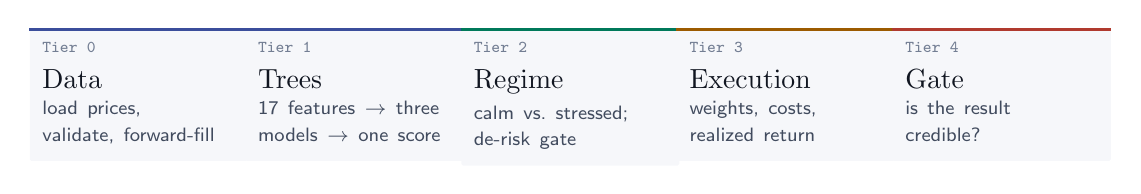
\begin{tikzpicture}[node distance=0mm]
\node[anchor=north west,inner sep=1.6mm,text width=24.5mm,fill=sunken,rounded corners=0.6pt] (n1) at (0.0mm,0) {{\ttfamily\fontsize{5.6}{7}\selectfont\color{muted}Tier 0}\\[0.4mm]{\dispfont\fontsize{10}{11}\selectfont\color{ink}Data}\\[0.8mm]{\sffamily\fontsize{6.6}{8.4}\selectfont\color{ink2}\begin{tabular}{@{}l@{}}load prices,\\[0.4mm]validate, forward-fill\end{tabular}}};
\draw[cA,line width=1.1pt] (n1.north west)--(n1.north east);
\node[anchor=north west,inner sep=1.6mm,text width=24.5mm,fill=sunken,rounded corners=0.6pt] (n3) at (27.4mm,0) {{\ttfamily\fontsize{5.6}{7}\selectfont\color{muted}Tier 1}\\[0.4mm]{\dispfont\fontsize{10}{11}\selectfont\color{ink}Trees}\\[0.8mm]{\sffamily\fontsize{6.6}{8.4}\selectfont\color{ink2}\begin{tabular}{@{}l@{}}17 features $\rightarrow$ three\\[0.4mm]models $\rightarrow$ one score\end{tabular}}};
\draw[cA,line width=1.1pt] (n3.north west)--(n3.north east);
\node[anchor=north west,inner sep=1.6mm,text width=24.5mm,fill=sunken,rounded corners=0.6pt] (n5) at (54.8mm,0) {{\ttfamily\fontsize{5.6}{7}\selectfont\color{muted}Tier 2}\\[0.4mm]{\dispfont\fontsize{10}{11}\selectfont\color{ink}Regime}\\[0.8mm]{\sffamily\fontsize{6.6}{8.4}\selectfont\color{ink2}\begin{tabular}{@{}l@{}}calm vs.\ stressed;\\[0.4mm]de-risk gate\end{tabular}}};
\draw[cB,line width=1.1pt] (n5.north west)--(n5.north east);
\node[anchor=north west,inner sep=1.6mm,text width=24.5mm,fill=sunken,rounded corners=0.6pt] (n7) at (82.2mm,0) {{\ttfamily\fontsize{5.6}{7}\selectfont\color{muted}Tier 3}\\[0.4mm]{\dispfont\fontsize{10}{11}\selectfont\color{ink}Execution}\\[0.8mm]{\sffamily\fontsize{6.6}{8.4}\selectfont\color{ink2}\begin{tabular}{@{}l@{}}weights, costs,\\[0.4mm]realized return\end{tabular}}};
\draw[cD,line width=1.1pt] (n7.north west)--(n7.north east);
\node[anchor=north west,inner sep=1.6mm,text width=24.5mm,fill=sunken,rounded corners=0.6pt] (n9) at (109.6mm,0) {{\ttfamily\fontsize{5.6}{7}\selectfont\color{muted}Tier 4}\\[0.4mm]{\dispfont\fontsize{10}{11}\selectfont\color{ink}Gate}\\[0.8mm]{\sffamily\fontsize{6.6}{8.4}\selectfont\color{ink2}\begin{tabular}{@{}l@{}}is the result\\[0.4mm]credible?\end{tabular}}};
\draw[cC,line width=1.1pt] (n9.north west)--(n9.north east);
\end{tikzpicture}\end{center}\vskip1mm
\note{Tier 2 deserves a caveat if asked: a two-state model only bisects volatility, so the usable output is a de-risk gate on the most stressed days, not a forecast.}\end{frame}
\eyebrow{The system}
\begin{frame}[t]{Five stages, each a function of the one before \textnormal{\itshape --- continued}}
\begin{columns}[T]\begin{column}{0.475\textwidth}\subhead{Two rules hold everywhere}
\bodytext{Missing prices are \str{carried forward, never backward}. Filling a gap with a later price would let the strategy act on information that did not exist yet.}
\vskip0.8mm
\bodytext{A signal formed on day T earns the return from day T to T+1. It is never credited with the move that produced it.}
\vskip0.8mm\end{column}\begin{column}{0.475\textwidth}\subhead{Why the last stage exists}
\bodytext{A backtest can always be made to look good by trying configurations until one works. Stage 4 measures how many were tried and raises the bar accordingly, so that a result which is merely the luckiest of many attempts does not pass.}
\vskip0.8mm\end{column}\end{columns}
\end{frame}
\eyebrow{The system}
\begin{frame}[t]{The models are never tested on what they were taught}
\begin{columns}[T]\begin{column}{0.40\textwidth}\bodytext{A model that is fitted and scored on the same period will always look skilful. This one is refitted repeatedly through history.}
\vskip0.8mm
\bodytext{Two years of data train three models — \mn{LightGBM}, \mn{XGBoost} and a random forest. They then predict the following quarter, which they have never seen. The window advances and everything is refitted.}
\vskip0.8mm
\bodytext{Over the sample this happens \str{38 times}. Every scored day was predicted by a model fitted only on days before it.}
\vskip0.8mm
\aside{The three models' predictions are averaged. Averaging different learners is more stable than trusting any single one.}\end{column}\begin{column}{0.575\textwidth}\begin{center}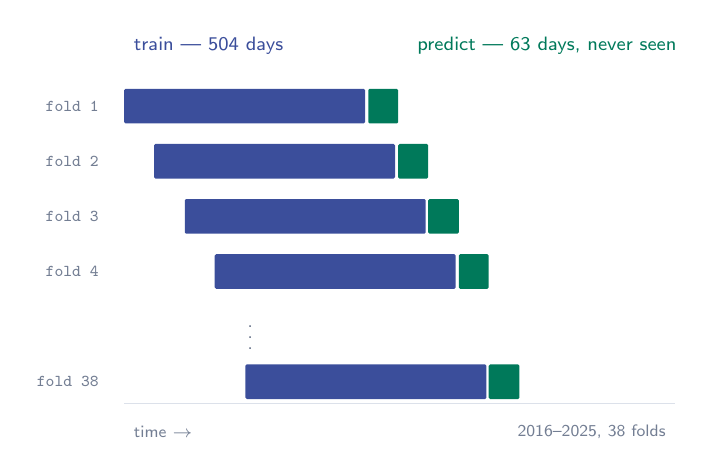
\begin{tikzpicture}[x=1mm,y=1mm]\fill[cA,rounded corners=0.5pt](0.0,0.0)rectangle(30.6,-4.4);\fill[cB,rounded corners=0.5pt](31.0,0.0)rectangle(34.8,-4.4);\node[anchor=east,font=\ttfamily\fontsize{6}{7}\selectfont,text=muted] at (-2,-2.2){fold 1};\fill[cA,rounded corners=0.5pt](3.8,-7.0)rectangle(34.4,-11.4);\fill[cB,rounded corners=0.5pt](34.8,-7.0)rectangle(38.6,-11.4);\node[anchor=east,font=\ttfamily\fontsize{6}{7}\selectfont,text=muted] at (-2,-9.2){fold 2};\fill[cA,rounded corners=0.5pt](7.7,-14.0)rectangle(38.3,-18.4);\fill[cB,rounded corners=0.5pt](38.6,-14.0)rectangle(42.5,-18.4);\node[anchor=east,font=\ttfamily\fontsize{6}{7}\selectfont,text=muted] at (-2,-16.2){fold 3};\fill[cA,rounded corners=0.5pt](11.5,-21.0)rectangle(42.1,-25.4);\fill[cB,rounded corners=0.5pt](42.5,-21.0)rectangle(46.3,-25.4);\node[anchor=east,font=\ttfamily\fontsize{6}{7}\selectfont,text=muted] at (-2,-23.2){fold 4};\node[font=\sffamily\fontsize{7}{8}\selectfont,text=muted] at (16,-30.5){$\vdots$};\fill[cA,rounded corners=0.5pt](15.4,-35.0)rectangle(46.0,-39.4);\fill[cB,rounded corners=0.5pt](46.3,-35.0)rectangle(50.2,-39.4);\node[anchor=east,font=\ttfamily\fontsize{6}{7}\selectfont,text=muted] at (-2,-37.2){fold 38};\node[anchor=west,font=\sffamily\fontsize{6.6}{8}\selectfont,text=cA] at (0,5.5){train --- 504 days};\node[anchor=west,font=\sffamily\fontsize{6.6}{8}\selectfont,text=cB] at (36,5.5){predict --- 63 days, never seen};\draw[hair,line width=0.4pt](0,-40.0)--(70,-40.0);\node[anchor=west,font=\sffamily\fontsize{6.2}{8}\selectfont,text=muted] at (0,-43.5){time $\rightarrow$};\node[anchor=east,font=\sffamily\fontsize{6.2}{8}\selectfont,text=muted] at (70,-43.5){2016--2025, 38 folds};\end{tikzpicture}\end{center}\vskip1mm\figcaption{Walk-forward estimation. Each row is one refit: the training window on the left, the out-of-sample quarter it then predicts on the right.}\end{column}\end{columns}
\note{This is the difference between a backtest and a demonstration. If a professor presses on look-ahead, this slide plus the forward-fill rule on slide 3 is the answer.}\end{frame}
\eyebrow{The system}
\begin{frame}[t]{The ranking does predict}
\begin{columns}[T]\begin{column}{0.40\textwidth}\bodytext{Skill is measured by the \str{information coefficient}: on each day, the correlation between the predicted ordering and what actually happened. Zero means the ranking is noise. In equities, 0.02–0.05 is a genuinely useful signal — the bar is low because so little of a single stock's daily move is predictable at all.}
\vskip0.8mm
\bodytext{The three-model average reaches \str{0.0511}, and ranks in the right direction on \str{69\%} of days across 2,333 days.}
\vskip0.8mm
\bodytext{This is the finding the rest of the deck has to be read against. \str{The signal is real.} Everything that follows is about what it costs to act on it.}\end{column}\begin{column}{0.575\textwidth}\begin{center}\setlength{\plotwidth}{74mm}\setlength{\plotheight}{42mm}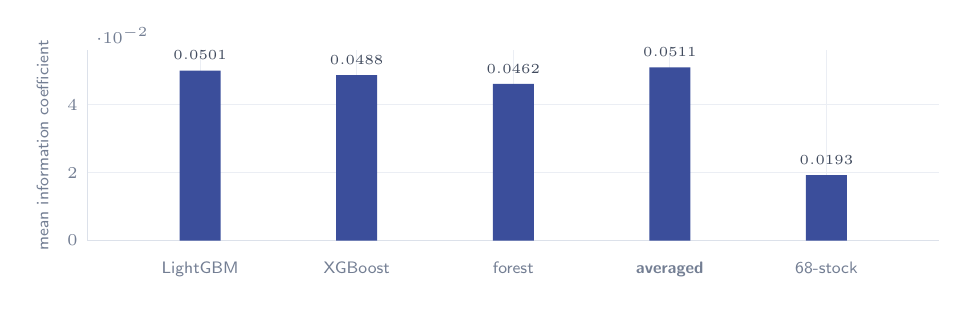
\begin{tikzpicture}\begin{axis}[qrtf,ybar,bar width=5.2mm,xtick={0,1,2,3,4},xticklabels={{LightGBM},{XGBoost},{forest},{\textbf{averaged}},{68-stock}},xtick style={draw=none},enlarge x limits=0.18,ylabel={mean information coefficient},ymin=0,legend style={draw=none,fill=none},legend to name=none,]\addplot[ybar,fill=cA,draw=none,nodes near coords,every node near coord/.append style={font=\ttfamily\fontsize{5.4}{6}\selectfont,color=ink2,/pgf/number format/.cd,fixed,precision=4},] coordinates{(0.0000,0.05009) (1.0000,0.04878) (2.0000,0.04621) (3.0000,0.05106) (4.0000,0.01929)};\addlegendentry{mean information coefficient}\end{axis}\end{tikzpicture}\end{center}\vskip1mm\figcaption{Mean daily cross-sectional rank IC by model, 500-name universe, 5-day target, 2,333 scored days. The rightmost bar is the earlier 68-stock universe for scale.}\end{column}\end{columns}
\note{If asked why IC rose 2.5× when the universe widened: the honest answer is that the 500-name universe contains a different and stronger cross-sectional effect, and slide 16 shows it is not confined to illiquid names.}\end{frame}
\eyebrow{Building a valid test}
\begin{frame}[t]{Phases 1 and 2 — the apparatus}
\begin{columns}[T]\begin{column}{0.40\textwidth}\bodytext{\str{Phase 1} ran the whole five-stage stack on \emph{simulated} prices for ten stocks, three of which were given a hidden upward drift. It confirmed that the machinery works end to end.}
\vskip0.8mm
\bodytext{It says nothing about markets. The simulator decided which stocks would win, so finding them demonstrates only that the search works — which is exactly what it was built to check.}
\vskip0.8mm
\bodytext{\str{Phase 2} replaced the simulation with real NSE data, replaced the simple momentum ranking with the tree models, and removed a look-ahead flaw in the regime detector, which had been fitted on the whole history at once.}\end{column}\begin{column}{0.575\textwidth}\begin{center}\setlength{\plotwidth}{74mm}\setlength{\plotheight}{42mm}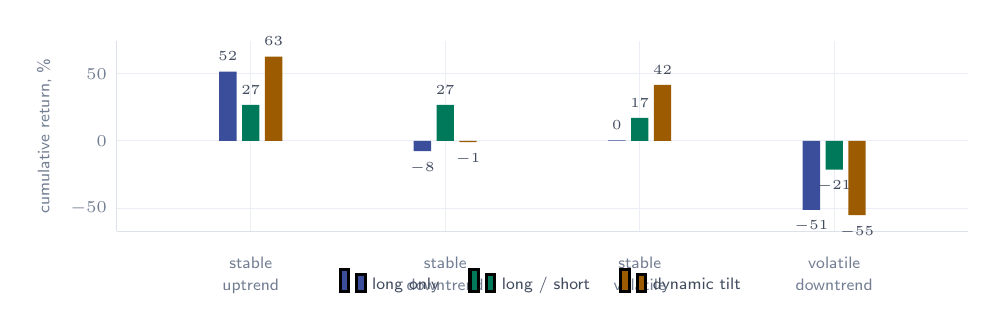
\begin{tikzpicture}\begin{axis}[qrtf,ybar,bar width=2.2mm,xtick={0,1,2,3},xticklabels={{\begin{tabular}{@{}c@{}}stable\\uptrend\end{tabular}},{\begin{tabular}{@{}c@{}}stable\\downtrend\end{tabular}},{\begin{tabular}{@{}c@{}}stable\\volatile\end{tabular}},{\begin{tabular}{@{}c@{}}volatile\\downtrend\end{tabular}}},xtick style={draw=none},enlarge x limits=0.23,ylabel={cumulative return, \%},legend style={at={(0.5,-0.16)},anchor=north,legend columns=-1,/tikz/every even column/.append style={column sep=3mm}},]\addplot[ybar,fill=cA,draw=none,nodes near coords,every node near coord/.append style={font=\ttfamily\fontsize{5.4}{6}\selectfont,color=ink2,/pgf/number format/.cd,fixed,precision=0},] coordinates{(0.0000,51.66000) (1.0000,-7.65000) (2.0000,0.37000) (3.0000,-51.31000)};\addlegendentry{long only}\addplot[ybar,fill=cB,draw=none,nodes near coords,every node near coord/.append style={font=\ttfamily\fontsize{5.4}{6}\selectfont,color=ink2,/pgf/number format/.cd,fixed,precision=0},] coordinates{(0.0000,26.86000) (1.0000,26.82000) (2.0000,17.16000) (3.0000,-21.45000)};\addlegendentry{long / short}\addplot[ybar,fill=cD,draw=none,nodes near coords,every node near coord/.append style={font=\ttfamily\fontsize{5.4}{6}\selectfont,color=ink2,/pgf/number format/.cd,fixed,precision=0},] coordinates{(0.0000,62.78000) (1.0000,-0.88000) (2.0000,41.78000) (3.0000,-55.32000)};\addlegendentry{dynamic tilt}\end{axis}\end{tikzpicture}\end{center}\vskip1mm\figcaption{Phase 1, cumulative return by simulated market regime and trading style. Synthetic data: a verification of pipeline mechanics, not an empirical result.}\end{column}\end{columns}
\note{Be direct that this chart is not evidence. It is included because the apparatus had to be verified before it could be trusted on real data.}\end{frame}
\eyebrow{Building a valid test}
\begin{frame}[t]{Phase 3 — the first collapse}
\begin{center}\setlength{\plotwidth}{124mm}\setlength{\plotheight}{31mm}\begin{tikzpicture}\begin{axis}[qrtf,xtick={0,1,2,3,4,5,6,7,8,9,10,11},xticklabels={{long only},{long/short},{dyn.\ tilt},{long only},{long/short},{dyn.\ tilt},{long only},{long/short},{dyn.\ tilt},{long only},{long/short},{dyn.\ tilt}},xtick style={draw=none},x tick label style={font=\sffamily\fontsize{6.2}{8}\selectfont,color=muted},enlarge x limits=0.06,ylabel={annualized Sharpe ratio},extra y ticks={0},extra y tick style={grid=major,grid style={hair,line width=0.5pt}},x tick label style={rotate=32,anchor=east,font=\sffamily\fontsize{5.8}{7}\selectfont,color=muted},]\draw[hair,line width=2.2pt,line cap=round](axis cs:0,1.6200)--(axis cs:0,0.4945);\draw[hair,line width=2.2pt,line cap=round](axis cs:1,1.8100)--(axis cs:1,-0.3659);\draw[hair,line width=2.2pt,line cap=round](axis cs:2,1.7400)--(axis cs:2,0.1842);\draw[hair,line width=2.2pt,line cap=round](axis cs:3,3.1700)--(axis cs:3,-6.9476);\draw[hair,line width=2.2pt,line cap=round](axis cs:4,8.0400)--(axis cs:4,-6.3367);\draw[hair,line width=2.2pt,line cap=round](axis cs:5,6.6600)--(axis cs:5,-7.3899);\draw[hair,line width=2.2pt,line cap=round](axis cs:6,6.2700)--(axis cs:6,-11.3169);\draw[hair,line width=2.2pt,line cap=round](axis cs:7,11.5000)--(axis cs:7,-10.2909);\draw[hair,line width=2.2pt,line cap=round](axis cs:8,11.3200)--(axis cs:8,-12.4324);\draw[hair,line width=2.2pt,line cap=round](axis cs:9,11.4200)--(axis cs:9,-17.4789);\draw[hair,line width=2.2pt,line cap=round](axis cs:10,16.2900)--(axis cs:10,-17.6102);\draw[hair,line width=2.2pt,line cap=round](axis cs:11,17.1600)--(axis cs:11,-21.1060);\addplot[only marks,mark=*,mark size=1.5pt,cA] coordinates{(0.0000,1.62000) (1.0000,1.81000) (2.0000,1.74000) (3.0000,3.17000) (4.0000,8.04000) (5.0000,6.66000) (6.0000,6.27000) (7.0000,11.50000) (8.0000,11.32000) (9.0000,11.42000) (10.0000,16.29000) (11.0000,17.16000)};\addplot[only marks,mark=*,mark size=1.5pt,cB] coordinates{(0.0000,0.49454) (2.0000,0.18425)};\addplot[only marks,mark=*,mark size=1.5pt,cC] coordinates{(1.0000,-0.36590) (3.0000,-6.94761) (4.0000,-6.33668) (5.0000,-7.38993) (6.0000,-11.31694) (7.0000,-10.29095) (8.0000,-12.43242) (9.0000,-17.47888) (10.0000,-17.61017) (11.0000,-21.10596)};\node[anchor=west,font=\ttfamily\fontsize{5.4}{6}\selectfont,text=ink2,xshift=1mm,yshift=1.1mm] at (axis cs:0,1.6200){1.62};\node[anchor=west,font=\ttfamily\fontsize{5.4}{6}\selectfont,text=cB,xshift=1mm,yshift=-1.4mm] at (axis cs:0,0.4945){0.49};\node[anchor=west,font=\ttfamily\fontsize{5.4}{6}\selectfont,text=ink2,xshift=1mm,yshift=1.1mm] at (axis cs:1,1.8100){1.81};\node[anchor=west,font=\ttfamily\fontsize{5.4}{6}\selectfont,text=cC,xshift=1mm,yshift=-1.4mm] at (axis cs:1,-0.3659){−0.37};\node[anchor=west,font=\ttfamily\fontsize{5.4}{6}\selectfont,text=ink2,xshift=1mm,yshift=1.1mm] at (axis cs:2,1.7400){1.74};\node[anchor=west,font=\ttfamily\fontsize{5.4}{6}\selectfont,text=cB,xshift=1mm,yshift=-1.4mm] at (axis cs:2,0.1842){0.18};\node[anchor=west,font=\ttfamily\fontsize{5.4}{6}\selectfont,text=ink2,xshift=1mm,yshift=0.0mm] at (axis cs:3,3.1700){3.17};\node[anchor=west,font=\ttfamily\fontsize{5.4}{6}\selectfont,text=cC,xshift=1mm,yshift=0.0mm] at (axis cs:3,-6.9476){−6.95};\node[anchor=west,font=\ttfamily\fontsize{5.4}{6}\selectfont,text=ink2,xshift=1mm,yshift=0.0mm] at (axis cs:4,8.0400){8.04};\node[anchor=west,font=\ttfamily\fontsize{5.4}{6}\selectfont,text=cC,xshift=1mm,yshift=0.0mm] at (axis cs:4,-6.3367){−6.34};\node[anchor=west,font=\ttfamily\fontsize{5.4}{6}\selectfont,text=ink2,xshift=1mm,yshift=0.0mm] at (axis cs:5,6.6600){6.66};\node[anchor=west,font=\ttfamily\fontsize{5.4}{6}\selectfont,text=cC,xshift=1mm,yshift=0.0mm] at (axis cs:5,-7.3899){−7.39};\node[anchor=west,font=\ttfamily\fontsize{5.4}{6}\selectfont,text=ink2,xshift=1mm,yshift=0.0mm] at (axis cs:6,6.2700){6.27};\node[anchor=west,font=\ttfamily\fontsize{5.4}{6}\selectfont,text=cC,xshift=1mm,yshift=0.0mm] at (axis cs:6,-11.3169){−11.32};\node[anchor=west,font=\ttfamily\fontsize{5.4}{6}\selectfont,text=ink2,xshift=1mm,yshift=0.0mm] at (axis cs:7,11.5000){11.50};\node[anchor=west,font=\ttfamily\fontsize{5.4}{6}\selectfont,text=cC,xshift=1mm,yshift=0.0mm] at (axis cs:7,-10.2909){−10.29};\node[anchor=west,font=\ttfamily\fontsize{5.4}{6}\selectfont,text=ink2,xshift=1mm,yshift=0.0mm] at (axis cs:8,11.3200){11.32};\node[anchor=west,font=\ttfamily\fontsize{5.4}{6}\selectfont,text=cC,xshift=1mm,yshift=0.0mm] at (axis cs:8,-12.4324){−12.43};\node[anchor=west,font=\ttfamily\fontsize{5.4}{6}\selectfont,text=ink2,xshift=1mm,yshift=0.0mm] at (axis cs:9,11.4200){11.42};\node[anchor=west,font=\ttfamily\fontsize{5.4}{6}\selectfont,text=cC,xshift=1mm,yshift=0.0mm] at (axis cs:9,-17.4789){−17.48};\node[anchor=west,font=\ttfamily\fontsize{5.4}{6}\selectfont,text=ink2,xshift=1mm,yshift=0.0mm] at (axis cs:10,16.2900){16.29};\node[anchor=west,font=\ttfamily\fontsize{5.4}{6}\selectfont,text=cC,xshift=1mm,yshift=0.0mm] at (axis cs:10,-17.6102){−17.61};\node[anchor=west,font=\ttfamily\fontsize{5.4}{6}\selectfont,text=ink2,xshift=1mm,yshift=0.0mm] at (axis cs:11,17.1600){17.16};\node[anchor=west,font=\ttfamily\fontsize{5.4}{6}\selectfont,text=cC,xshift=1mm,yshift=0.0mm] at (axis cs:11,-21.1060){−21.11};\node[font=\sffamily\fontsize{6.2}{8}\selectfont,text=muted,anchor=north,yshift=-6.6mm] at (axis cs:1.0,\pgfkeysvalueof{/pgfplots/ymin}){daily};\node[font=\sffamily\fontsize{6.2}{8}\selectfont,text=muted,anchor=north,yshift=-6.6mm] at (axis cs:4.0,\pgfkeysvalueof{/pgfplots/ymin}){hourly};\node[font=\sffamily\fontsize{6.2}{8}\selectfont,text=muted,anchor=north,yshift=-6.6mm] at (axis cs:7.0,\pgfkeysvalueof{/pgfplots/ymin}){every 30 min};\node[font=\sffamily\fontsize{6.2}{8}\selectfont,text=muted,anchor=north,yshift=-6.6mm] at (axis cs:10.0,\pgfkeysvalueof{/pgfplots/ymin}){every 15 min};\end{axis}\end{tikzpicture}\end{center}\figcaption{Each line runs from a configuration's Sharpe before costs to its Sharpe after costs. Gross values from the Phase 3 record; net values recomputed from the 12-cell ledger. 68 stocks, 2018–2025.}\vskip2.2mm\begin{columns}[T]\begin{column}{0.475\textwidth}\bodytext{Phase 3 charged the actual Indian statutory cost of trading — securities transaction tax, exchange and regulator fees, stamp duty, GST and brokerage — about \str{14.7 basis points each time a position is opened or closed} (a basis point is one hundredth of one percent).}\end{column}\begin{column}{0.475\textwidth}\end{column}\end{columns}
\note{The length of each line is the cost. Note the ordering inverts: the fastest strategies look best before costs and worst after. The conclusion carried into Phase 4 was that 68 stocks was too small a universe.}\end{frame}
\eyebrow{Building a valid test}
\begin{frame}[t]{Phase 3 — the first collapse \textnormal{\itshape --- continued}}
\begin{columns}[T]\begin{column}{0.475\textwidth}\bodytext{Faster trading means more of those charges. Every intraday configuration went to \str{−100\%}: the strategy trades so often that the fees exceed the edge with certainty, not by bad luck. The only survivor was the daily long-only book, at a Sharpe ratio of 0.57 — a measure of return per unit of risk, where above 1 is good and below 0 loses money — which still fell short of the credibility gate.}\end{column}\begin{column}{0.475\textwidth}\end{column}\end{columns}
\end{frame}
\eyebrow{Phase 4b}
\begin{frame}[t]{Widening the universe from 68 stocks to 500}
\begin{columns}[T]\begin{column}{0.40\textwidth}\bodytext{Standard portfolio theory says that skill of a given quality applied to more independent bets produces a better risk-adjusted return, scaling roughly with the square root of the number of bets. Going from 68 names to 500 predicts an improvement of about \str{2.7×}, against the \str{1.5×} needed to pass.}
\vskip0.8mm
\bodytext{Testing that required rebuilding the dataset from the exchange's public daily archive as a \str{point-in-time} index membership: a company that belonged to the index in 2017 and later collapsed is still present in 2017.}
\vskip0.8mm\end{column}\begin{column}{0.575\textwidth}\begin{center}\setlength{\plotwidth}{74mm}\setlength{\plotheight}{42mm}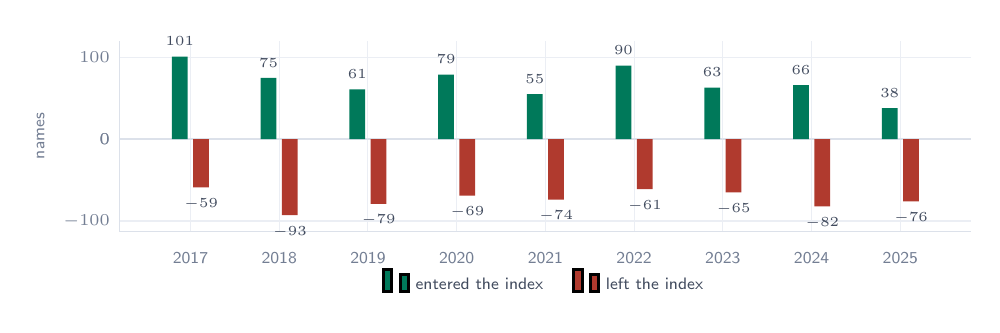
\begin{tikzpicture}\begin{axis}[qrtf,ybar,bar width=2.0mm,xtick={0,1,2,3,4,5,6,7,8},xticklabels={{2017},{2018},{2019},{2020},{2021},{2022},{2023},{2024},{2025}},xtick style={draw=none},enlarge x limits=0.10,ylabel={names},extra y ticks={0},extra y tick style={grid=major,grid style={hair,line width=0.5pt}},legend style={at={(0.5,-0.16)},anchor=north,legend columns=-1,/tikz/every even column/.append style={column sep=3mm}},]\addplot[ybar,fill=cB,draw=none,nodes near coords,every node near coord/.append style={font=\ttfamily\fontsize{5.4}{6}\selectfont,color=ink2,/pgf/number format/.cd,fixed,precision=0},] coordinates{(0.0000,101.00000) (1.0000,75.00000) (2.0000,61.00000) (3.0000,79.00000) (4.0000,55.00000) (5.0000,90.00000) (6.0000,63.00000) (7.0000,66.00000) (8.0000,38.00000)};\addlegendentry{entered the index}\addplot[ybar,fill=cC,draw=none,nodes near coords,every node near coord/.append style={font=\ttfamily\fontsize{5.4}{6}\selectfont,color=ink2,/pgf/number format/.cd,fixed,precision=0},] coordinates{(0.0000,-59.00000) (1.0000,-93.00000) (2.0000,-79.00000) (3.0000,-69.00000) (4.0000,-74.00000) (5.0000,-61.00000) (6.0000,-65.00000) (7.0000,-82.00000) (8.0000,-76.00000)};\addlegendentry{left the index}\end{axis}\end{tikzpicture}\end{center}\vskip1mm\figcaption{Membership churn per year, computed from the point-in-time universe mask. Names entering above the line, names leaving below.}\end{column}\end{columns}
\note{If asked why churn matters: every name below the line is a company a survivorship-biased dataset would have silently deleted from its own past.}\end{frame}
\eyebrow{Phase 4b}
\begin{frame}[t]{Widening the universe from 68 stocks to 500 \textnormal{\itshape --- continued}}
\begin{columns}[T]\begin{column}{0.475\textwidth}\bodytext{Without this, a backtest quietly restricts itself to firms that survived — which is information nobody had at the time. Over the sample, \str{1,035 different companies} passed through a universe that only ever holds 500 at once.}\end{column}\begin{column}{0.475\textwidth}\end{column}\end{columns}
\end{frame}
\eyebrow{Phase 4b}
\begin{frame}[t]{Phase 4b — two of three configurations passed}
\begin{center}\setlength{\plotwidth}{124mm}\setlength{\plotheight}{37mm}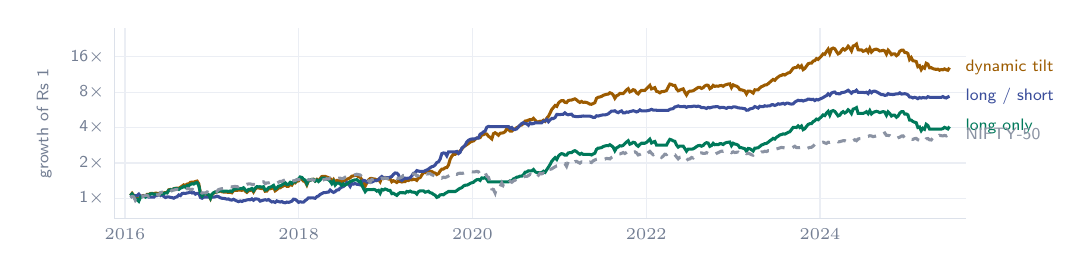
\begin{tikzpicture}\begin{axis}[qrtf,ymode=log,log basis y=10,ytick={1,2,4,8,16},yticklabels={1$\times$,2$\times$,4$\times$,8$\times$,16$\times$},xtick={2016,2018,2020,2022,2024},xticklabel style={/pgf/number format/1000 sep=},ylabel={growth of Rs 1},enlarge x limits=0.02,]\addplot[cD,line width=1.1pt,mark=none] coordinates{(2016.0630,1.05998) (2016.0822,1.10402) (2016.1014,1.05920) (2016.1205,0.98985) (2016.1397,0.99669) (2016.1589,0.97033) (2016.1781,1.04203) (2016.1973,1.04517) (2016.2164,1.05698) (2016.2356,1.04184) (2016.2548,1.08028) (2016.2740,1.07838) (2016.2932,1.09963) (2016.3123,1.10417) (2016.3315,1.09589) (2016.3507,1.10721) (2016.3699,1.10446) (2016.3890,1.10165) (2016.4082,1.10441) (2016.4274,1.11423) (2016.4466,1.11438) (2016.4658,1.11999) (2016.4849,1.12191) (2016.5041,1.18306) (2016.5233,1.19213) (2016.5425,1.17578) (2016.5616,1.20869) (2016.5808,1.21775) (2016.6000,1.22244) (2016.6192,1.21713) (2016.6384,1.24386) (2016.6575,1.27216) (2016.6767,1.30275) (2016.6959,1.28335) (2016.7151,1.32398) (2016.7342,1.32857) (2016.7534,1.36732) (2016.7726,1.37660) (2016.7918,1.37326) (2016.8110,1.39205) (2016.8301,1.40309) (2016.8493,1.33025) (2016.8685,1.10833) (2016.8877,1.05320) (2016.9068,1.08857) (2016.9260,1.08681) (2016.9452,1.08245) (2016.9644,1.06366) (2016.9836,0.99484) (2017.0000,1.07227) (2017.0192,1.10702) (2017.0384,1.12746) (2017.0575,1.13404) (2017.0767,1.14296) (2017.0959,1.15912) (2017.1151,1.13919) (2017.1342,1.13221) (2017.1534,1.13215) (2017.1726,1.12857) (2017.1918,1.12566) (2017.2110,1.12786) (2017.2301,1.11525) (2017.2493,1.16470) (2017.2685,1.16856) (2017.2877,1.16781) (2017.3068,1.17829) (2017.3260,1.17629) (2017.3452,1.17029) (2017.3644,1.19668) (2017.3836,1.15385) (2017.4027,1.12564) (2017.4219,1.16417) (2017.4411,1.16724) (2017.4603,1.19296) (2017.4795,1.13354) (2017.4986,1.19843) (2017.5178,1.23524) (2017.5370,1.22850) (2017.5562,1.21690) (2017.5753,1.21079) (2017.5945,1.22501) (2017.6137,1.14999) (2017.6329,1.15381) (2017.6521,1.20569) (2017.6712,1.20785) (2017.6904,1.21786) (2017.7096,1.24537) (2017.7288,1.16079) (2017.7479,1.18798) (2017.7671,1.23005) (2017.7863,1.23135) (2017.8055,1.25732) (2017.8247,1.27936) (2017.8438,1.30289) (2017.8630,1.26603) (2017.8822,1.26812) (2017.9014,1.32067) (2017.9205,1.29740) (2017.9397,1.36875) (2017.9589,1.35405) (2017.9781,1.40453) (2017.9973,1.40605) (2018.0164,1.46867) (2018.0356,1.45288) (2018.0548,1.40280) (2018.0740,1.39053) (2018.0932,1.30243) (2018.1123,1.41140) (2018.1315,1.42288) (2018.1507,1.44958) (2018.1699,1.45597) (2018.1890,1.40648) (2018.2082,1.45236) (2018.2274,1.41311) (2018.2466,1.47073) (2018.2658,1.53357) (2018.2849,1.54124) (2018.3041,1.54036) (2018.3233,1.51793) (2018.3425,1.49835) (2018.3616,1.47643) (2018.3808,1.39175) (2018.4000,1.44840) (2018.4192,1.35421) (2018.4384,1.42032) (2018.4575,1.42203) (2018.4767,1.41709) (2018.4959,1.38013) (2018.5151,1.42940) (2018.5342,1.41129) (2018.5534,1.45453) (2018.5726,1.47250) (2018.5918,1.49743) (2018.6110,1.54316) (2018.6301,1.55339) (2018.6493,1.57281) (2018.6685,1.57046) (2018.6877,1.52201) (2018.7068,1.52087) (2018.7260,1.43508) (2018.7452,1.35722) (2018.7644,1.27093) (2018.7836,1.35602) (2018.8027,1.43260) (2018.8219,1.47491) (2018.8411,1.47701) (2018.8603,1.46307) (2018.8795,1.45840) (2018.8986,1.42162) (2018.9178,1.45007) (2018.9370,1.38565) (2018.9562,1.50151) (2018.9753,1.47547) (2018.9945,1.50565) (2019.0137,1.48886) (2019.0329,1.46191) (2019.0521,1.46804) (2019.0712,1.38406) (2019.0904,1.41256) (2019.1096,1.39288) (2019.1288,1.36513) (2019.1479,1.39941) (2019.1671,1.39294) (2019.1863,1.37866) (2019.2055,1.39031) (2019.2247,1.38921) (2019.2438,1.43139) (2019.2630,1.41935) (2019.2822,1.44677) (2019.3014,1.43659) (2019.3205,1.45536) (2019.3397,1.44917) (2019.3589,1.42233) (2019.3781,1.48864) (2019.3973,1.50204) (2019.4164,1.58210) (2019.4356,1.66371) (2019.4548,1.65502) (2019.4740,1.70383) (2019.4932,1.73170) (2019.5123,1.69430) (2019.5315,1.69295) (2019.5507,1.65589) (2019.5699,1.64216) (2019.5890,1.59548) (2019.6082,1.62380) (2019.6274,1.70971) (2019.6466,1.77362) (2019.6658,1.77802) (2019.6849,1.82143) (2019.7041,1.82695) (2019.7233,1.91938) (2019.7425,2.15287) (2019.7616,2.28090) (2019.7808,2.37744) (2019.8000,2.36966) (2019.8192,2.42975) (2019.8384,2.46689) (2019.8575,2.53014) (2019.8767,2.62719) (2019.8959,2.73247) (2019.9151,2.80071) (2019.9342,2.86173) (2019.9534,2.92820) (2019.9726,3.00694) (2019.9918,3.05205) (2020.0110,3.08185) (2020.0301,3.17804) (2020.0493,3.25941) (2020.0685,3.27622) (2020.0877,3.28841) (2020.1068,3.47061) (2020.1260,3.48071) (2020.1452,3.54410) (2020.1644,3.52459) (2020.1836,3.37373) (2020.2027,3.30303) (2020.2219,3.20623) (2020.2411,3.55282) (2020.2603,3.61646) (2020.2795,3.53962) (2020.2986,3.44439) (2020.3178,3.57851) (2020.3370,3.59467) (2020.3562,3.61722) (2020.3753,3.69589) (2020.3945,3.92028) (2020.4137,3.84341) (2020.4329,3.73454) (2020.4521,3.73724) (2020.4712,3.85262) (2020.4904,3.89747) (2020.5096,3.99944) (2020.5288,4.06452) (2020.5479,4.18127) (2020.5671,4.21185) (2020.5863,4.34839) (2020.6055,4.54730) (2020.6247,4.56542) (2020.6438,4.63063) (2020.6630,4.68624) (2020.6822,4.66502) (2020.7014,4.79674) (2020.7205,4.62601) (2020.7397,4.47156) (2020.7589,4.47859) (2020.7781,4.52951) (2020.7973,4.51189) (2020.8164,4.62233) (2020.8356,4.52848) (2020.8548,4.81111) (2020.8740,4.98744) (2020.8932,5.32365) (2020.9123,5.70462) (2020.9315,5.92533) (2020.9507,6.16690) (2020.9699,6.06098) (2020.9890,6.46096) (2021.0055,6.64980) (2021.0247,6.79394) (2021.0438,6.79805) (2021.0630,6.57005) (2021.0822,6.52748) (2021.1014,6.78185) (2021.1205,6.84579) (2021.1397,6.85759) (2021.1589,6.95287) (2021.1781,7.03012) (2021.1973,6.88989) (2021.2164,6.69637) (2021.2356,6.55119) (2021.2548,6.68089) (2021.2740,6.55582) (2021.2932,6.57922) (2021.3123,6.55685) (2021.3315,6.45651) (2021.3507,6.32955) (2021.3699,6.31991) (2021.3890,6.41429) (2021.4082,6.51974) (2021.4274,7.09641) (2021.4466,7.25278) (2021.4658,7.29313) (2021.4849,7.36667) (2021.5041,7.52698) (2021.5233,7.60931) (2021.5425,7.68504) (2021.5616,7.70069) (2021.5808,7.91813) (2021.6000,7.81806) (2021.6192,7.60333) (2021.6384,7.11340) (2021.6575,7.46692) (2021.6767,7.56844) (2021.6959,7.80663) (2021.7151,7.79914) (2021.7342,7.80402) (2021.7534,8.05784) (2021.7726,8.37248) (2021.7918,8.57119) (2021.8110,8.05193) (2021.8301,8.17136) (2021.8493,8.40508) (2021.8685,8.30973) (2021.8877,7.90093) (2021.9068,7.74204) (2021.9260,8.08540) (2021.9452,8.30886) (2021.9644,8.30882) (2021.9836,8.28975) (2022.0027,8.55221) (2022.0219,8.83505) (2022.0411,9.14667) (2022.0603,8.54130) (2022.0795,8.64283) (2022.0986,8.75149) (2022.1178,8.14245) (2022.1370,8.07104) (2022.1562,7.91136) (2022.1753,8.08767) (2022.1945,8.10541) (2022.2137,8.15786) (2022.2329,8.27220) (2022.2521,8.84938) (2022.2712,9.38187) (2022.2904,9.31304) (2022.3096,9.14551) (2022.3288,9.15544) (2022.3479,8.53994) (2022.3671,8.22378) (2022.3863,8.33445) (2022.4055,8.46111) (2022.4247,8.54803) (2022.4438,7.99129) (2022.4630,7.58121) (2022.4822,8.01456) (2022.5014,8.17398) (2022.5205,8.18476) (2022.5397,8.24228) (2022.5589,8.41414) (2022.5781,8.59618) (2022.5973,8.78125) (2022.6164,8.80885) (2022.6356,8.61747) (2022.6548,8.74207) (2022.6740,9.04676) (2022.6932,9.18290) (2022.7123,9.16457) (2022.7315,8.57295) (2022.7507,8.73643) (2022.7699,9.14123) (2022.7890,8.97517) (2022.8082,9.03384) (2022.8274,8.99224) (2022.8466,9.09727) (2022.8658,9.12656) (2022.8849,8.99157) (2022.9041,9.20068) (2022.9233,9.29281) (2022.9425,9.38969) (2022.9616,9.43018) (2022.9808,8.76443) (2023.0000,9.23385) (2023.0192,9.08646) (2023.0384,9.01238) (2023.0575,8.81975) (2023.0767,8.40266) (2023.0959,8.39190) (2023.1151,8.29105) (2023.1342,8.19986) (2023.1534,7.73099) (2023.1726,8.17418) (2023.1918,8.18426) (2023.2110,8.04901) (2023.2301,7.87199) (2023.2493,8.39359) (2023.2685,8.38275) (2023.2877,8.39560) (2023.3068,8.69144) (2023.3260,8.92121) (2023.3452,9.03237) (2023.3644,9.21268) (2023.3836,9.23470) (2023.4027,9.45533) (2023.4219,9.72746) (2023.4411,10.00306) (2023.4603,10.27807) (2023.4795,10.10112) (2023.4986,10.49898) (2023.5178,10.77901) (2023.5370,11.02541) (2023.5562,11.13556) (2023.5753,11.32505) (2023.5945,11.20315) (2023.6137,11.45127) (2023.6329,11.67196) (2023.6521,11.76686) (2023.6712,12.24736) (2023.6904,12.81198) (2023.7096,12.96385) (2023.7288,12.98762) (2023.7479,13.47088) (2023.7671,13.00748) (2023.7863,13.42002) (2023.8055,12.46382) (2023.8247,12.74379) (2023.8438,13.33907) (2023.8630,13.96527) (2023.8822,14.12765) (2023.9014,14.13274) (2023.9205,14.72096) (2023.9397,14.85812) (2023.9589,15.45881) (2023.9781,15.21068) (2023.9973,15.74811) (2024.0164,16.27711) (2024.0356,16.96273) (2024.0548,16.83125) (2024.0740,17.77619) (2024.0932,18.59453) (2024.1123,17.08855) (2024.1315,18.68367) (2024.1507,19.00866) (2024.1699,18.74187) (2024.1890,17.75299) (2024.2082,16.95784) (2024.2274,17.27044) (2024.2466,18.14433) (2024.2658,18.74556) (2024.2849,18.28477) (2024.3041,18.76379) (2024.3233,19.70173) (2024.3425,19.00957) (2024.3616,17.98602) (2024.3808,19.78503) (2024.4000,19.98050) (2024.4192,20.53788) (2024.4384,18.37535) (2024.4575,18.29593) (2024.4767,18.35235) (2024.4959,17.82639) (2024.5151,18.02885) (2024.5342,18.43872) (2024.5534,17.60564) (2024.5726,18.94252) (2024.5918,17.59727) (2024.6110,18.22694) (2024.6301,18.50414) (2024.6493,18.61218) (2024.6685,18.34099) (2024.6877,17.95040) (2024.7068,18.02847) (2024.7260,18.18487) (2024.7452,17.95248) (2024.7644,16.87759) (2024.7836,18.22961) (2024.8027,17.57785) (2024.8219,16.71374) (2024.8411,16.98429) (2024.8603,16.98043) (2024.8795,16.36697) (2024.8986,16.76885) (2024.9178,17.85626) (2024.9370,18.21242) (2024.9562,18.25092) (2024.9753,17.42798) (2024.9945,17.40019) (2025.0110,17.06208) (2025.0301,15.19819) (2025.0493,15.77801) (2025.0685,14.81940) (2025.0877,14.74396) (2025.1068,14.59910) (2025.1260,13.21146) (2025.1452,13.43093) (2025.1644,12.45538) (2025.1836,13.10458) (2025.2027,12.82342) (2025.2219,14.11115) (2025.2411,13.89467) (2025.2603,12.91030) (2025.2795,12.95159) (2025.2986,12.71143) (2025.3178,12.56887) (2025.3370,12.53137) (2025.3562,12.57267) (2025.3753,12.30868) (2025.3945,12.48450) (2025.4137,12.41321) (2025.4329,12.64052) (2025.4521,12.42354) (2025.4712,12.30386) (2025.4904,12.94714)};\node[anchor=west,font=\sffamily\fontsize{6.4}{8}\selectfont,text=cD,xshift=0.8mm] at (axis cs:2025.4904,12.94714){dynamic tilt};\addplot[cA,line width=1.1pt,mark=none] coordinates{(2016.0630,1.01951) (2016.0822,1.04447) (2016.1014,1.04090) (2016.1205,1.05710) (2016.1397,1.05673) (2016.1589,1.08802) (2016.1781,1.04341) (2016.1973,1.04261) (2016.2164,1.04219) (2016.2356,1.05127) (2016.2548,1.03607) (2016.2740,1.02575) (2016.2932,1.02525) (2016.3123,1.02432) (2016.3315,1.02308) (2016.3507,1.05376) (2016.3699,1.05558) (2016.3890,1.07538) (2016.4082,1.05464) (2016.4274,1.07522) (2016.4466,1.03963) (2016.4658,1.01691) (2016.4849,1.02820) (2016.5041,1.02917) (2016.5233,1.01994) (2016.5425,1.01520) (2016.5616,1.00379) (2016.5808,1.02189) (2016.6000,1.03129) (2016.6192,1.06969) (2016.6384,1.05550) (2016.6575,1.09972) (2016.6767,1.10581) (2016.6959,1.10085) (2016.7151,1.11164) (2016.7342,1.11815) (2016.7534,1.13115) (2016.7726,1.11085) (2016.7918,1.12313) (2016.8110,1.08715) (2016.8301,1.10360) (2016.8493,1.10366) (2016.8685,1.01833) (2016.8877,1.00298) (2016.9068,1.02355) (2016.9260,1.02355) (2016.9452,1.02355) (2016.9644,1.02331) (2016.9836,1.02175) (2017.0000,1.02245) (2017.0192,1.02422) (2017.0384,1.03054) (2017.0575,1.04330) (2017.0767,1.03394) (2017.0959,1.01287) (2017.1151,1.00241) (2017.1342,1.00069) (2017.1534,0.99495) (2017.1726,0.98433) (2017.1918,0.99054) (2017.2110,0.97111) (2017.2301,0.96705) (2017.2493,0.98195) (2017.2685,0.96508) (2017.2877,0.94968) (2017.3068,0.93805) (2017.3260,0.95027) (2017.3452,0.94066) (2017.3644,0.95574) (2017.3836,0.95899) (2017.4027,0.97013) (2017.4219,0.97523) (2017.4411,0.97228) (2017.4603,0.99087) (2017.4795,0.96432) (2017.4986,0.99035) (2017.5178,0.98792) (2017.5370,0.98189) (2017.5562,0.94762) (2017.5753,0.95647) (2017.5945,0.96668) (2017.6137,0.97392) (2017.6329,0.96471) (2017.6521,0.97734) (2017.6712,0.95338) (2017.6904,0.93176) (2017.7096,0.93682) (2017.7288,0.92396) (2017.7479,0.95129) (2017.7671,0.93819) (2017.7863,0.93105) (2017.8055,0.93882) (2017.8247,0.92287) (2017.8438,0.91718) (2017.8630,0.93037) (2017.8822,0.92406) (2017.9014,0.93370) (2017.9205,0.94633) (2017.9397,0.98483) (2017.9589,0.98043) (2017.9781,0.95720) (2017.9973,0.92527) (2018.0164,0.93570) (2018.0356,0.92969) (2018.0548,0.92939) (2018.0740,0.95788) (2018.0932,0.97940) (2018.1123,1.01054) (2018.1315,1.00758) (2018.1507,1.01136) (2018.1699,1.00840) (2018.1890,1.00132) (2018.2082,1.03568) (2018.2274,1.04749) (2018.2466,1.07946) (2018.2658,1.09810) (2018.2849,1.11744) (2018.3041,1.11805) (2018.3233,1.12708) (2018.3425,1.13042) (2018.3616,1.17682) (2018.3808,1.14674) (2018.4000,1.12374) (2018.4192,1.14024) (2018.4384,1.17712) (2018.4575,1.18091) (2018.4767,1.22163) (2018.4959,1.24789) (2018.5151,1.26052) (2018.5342,1.31376) (2018.5534,1.36456) (2018.5726,1.32482) (2018.5918,1.26306) (2018.6110,1.34377) (2018.6301,1.32228) (2018.6493,1.33832) (2018.6685,1.31710) (2018.6877,1.31356) (2018.7068,1.30263) (2018.7260,1.37917) (2018.7452,1.42319) (2018.7644,1.41167) (2018.7836,1.37738) (2018.8027,1.37738) (2018.8219,1.37738) (2018.8411,1.37738) (2018.8603,1.39764) (2018.8795,1.41964) (2018.8986,1.41912) (2018.9178,1.44375) (2018.9370,1.49820) (2018.9562,1.53588) (2018.9753,1.49783) (2018.9945,1.49643) (2019.0137,1.50236) (2019.0329,1.49592) (2019.0521,1.51827) (2019.0712,1.53553) (2019.0904,1.60078) (2019.1096,1.64496) (2019.1288,1.63936) (2019.1479,1.58675) (2019.1671,1.45735) (2019.1863,1.42226) (2019.2055,1.45960) (2019.2247,1.48799) (2019.2438,1.48032) (2019.2630,1.48578) (2019.2822,1.49538) (2019.3014,1.55368) (2019.3205,1.63490) (2019.3397,1.65214) (2019.3589,1.72247) (2019.3781,1.70786) (2019.3973,1.69396) (2019.4164,1.69396) (2019.4356,1.69396) (2019.4548,1.72176) (2019.4740,1.74128) (2019.4932,1.77638) (2019.5123,1.82166) (2019.5315,1.85988) (2019.5507,1.87485) (2019.5699,1.92443) (2019.5890,2.01703) (2019.6082,2.04527) (2019.6274,2.15914) (2019.6466,2.40091) (2019.6658,2.43561) (2019.6849,2.42201) (2019.7041,2.30082) (2019.7233,2.48373) (2019.7425,2.48373) (2019.7616,2.48373) (2019.7808,2.48373) (2019.8000,2.48373) (2019.8192,2.50850) (2019.8384,2.40498) (2019.8575,2.46549) (2019.8767,2.67298) (2019.8959,2.74682) (2019.9151,2.83362) (2019.9342,3.02519) (2019.9534,3.11844) (2019.9726,3.17521) (2019.9918,3.19992) (2020.0110,3.20003) (2020.0301,3.20881) (2020.0493,3.26199) (2020.0685,3.26075) (2020.0877,3.51760) (2020.1068,3.57226) (2020.1260,3.67925) (2020.1452,3.73447) (2020.1644,4.02506) (2020.1836,4.09431) (2020.2027,4.08230) (2020.2219,4.08230) (2020.2411,4.08230) (2020.2603,4.08230) (2020.2795,4.08230) (2020.2986,4.08230) (2020.3178,4.08230) (2020.3370,4.08230) (2020.3562,4.08230) (2020.3753,4.08230) (2020.3945,4.08230) (2020.4137,4.08230) (2020.4329,3.94507) (2020.4521,4.00963) (2020.4712,3.85880) (2020.4904,3.85225) (2020.5096,3.90671) (2020.5288,4.04868) (2020.5479,4.20554) (2020.5671,4.33619) (2020.5863,4.40256) (2020.6055,4.32568) (2020.6247,4.31639) (2020.6438,4.18940) (2020.6630,4.38735) (2020.6822,4.30384) (2020.7014,4.32780) (2020.7205,4.40001) (2020.7397,4.39705) (2020.7589,4.39705) (2020.7781,4.39705) (2020.7973,4.39705) (2020.8164,4.54535) (2020.8356,4.55589) (2020.8548,4.68540) (2020.8740,4.48809) (2020.8932,4.65990) (2020.9123,4.78184) (2020.9315,4.77792) (2020.9507,4.88095) (2020.9699,5.17861) (2020.9890,5.17061) (2021.0055,5.15411) (2021.0247,5.19278) (2021.0438,5.19031) (2021.0630,5.34450) (2021.0822,5.20332) (2021.1014,5.13920) (2021.1205,5.18451) (2021.1397,5.20341) (2021.1589,5.01001) (2021.1781,4.98675) (2021.1973,4.95719) (2021.2164,4.96110) (2021.2356,4.99206) (2021.2548,4.99585) (2021.2740,5.02223) (2021.2932,5.00751) (2021.3123,5.00751) (2021.3315,5.00751) (2021.3507,5.00751) (2021.3699,4.95324) (2021.3890,4.87714) (2021.4082,4.89144) (2021.4274,5.04368) (2021.4466,5.01725) (2021.4658,5.06339) (2021.4849,5.10788) (2021.5041,5.13290) (2021.5233,5.12477) (2021.5425,5.16781) (2021.5616,5.23592) (2021.5808,5.37850) (2021.6000,5.52645) (2021.6192,5.51793) (2021.6384,5.56127) (2021.6575,5.43234) (2021.6767,5.36229) (2021.6959,5.47475) (2021.7151,5.54957) (2021.7342,5.34734) (2021.7534,5.33721) (2021.7726,5.43526) (2021.7918,5.40064) (2021.8110,5.47882) (2021.8301,5.51145) (2021.8493,5.56764) (2021.8685,5.51214) (2021.8877,5.43650) (2021.9068,5.50036) (2021.9260,5.66154) (2021.9452,5.55621) (2021.9644,5.55621) (2021.9836,5.55621) (2022.0027,5.55943) (2022.0219,5.58463) (2022.0411,5.64268) (2022.0603,5.72127) (2022.0795,5.63441) (2022.0986,5.63287) (2022.1178,5.61990) (2022.1370,5.60343) (2022.1562,5.60343) (2022.1753,5.60343) (2022.1945,5.60343) (2022.2137,5.60343) (2022.2329,5.60343) (2022.2521,5.60572) (2022.2712,5.72456) (2022.2904,5.77461) (2022.3096,5.79844) (2022.3288,5.99314) (2022.3479,6.03449) (2022.3671,6.12129) (2022.3863,6.04581) (2022.4055,6.04581) (2022.4247,6.04581) (2022.4438,6.05098) (2022.4630,5.95420) (2022.4822,6.04230) (2022.5014,6.04230) (2022.5205,6.04230) (2022.5397,6.08170) (2022.5589,6.08504) (2022.5781,6.04566) (2022.5973,6.09467) (2022.6164,6.03384) (2022.6356,5.91877) (2022.6548,5.93136) (2022.6740,5.89370) (2022.6932,5.82500) (2022.7123,5.94165) (2022.7315,5.88416) (2022.7507,5.95278) (2022.7699,5.99720) (2022.7890,6.01144) (2022.8082,6.04092) (2022.8274,6.01464) (2022.8466,5.89735) (2022.8658,5.95618) (2022.8849,5.95170) (2022.9041,5.89227) (2022.9233,5.83475) (2022.9425,5.94123) (2022.9616,5.93518) (2022.9808,5.90166) (2023.0000,5.99447) (2023.0192,5.99927) (2023.0384,5.96551) (2023.0575,5.88865) (2023.0767,5.87123) (2023.0959,5.85719) (2023.1151,5.82085) (2023.1342,5.79258) (2023.1534,5.62218) (2023.1726,5.62894) (2023.1918,5.76855) (2023.2110,5.81326) (2023.2301,5.86283) (2023.2493,6.03899) (2023.2685,5.96174) (2023.2877,5.86930) (2023.3068,6.07349) (2023.3260,6.03635) (2023.3452,6.03308) (2023.3644,6.13479) (2023.3836,6.08517) (2023.4027,6.11779) (2023.4219,6.12287) (2023.4411,6.25689) (2023.4603,6.26183) (2023.4795,6.17450) (2023.4986,6.25050) (2023.5178,6.38396) (2023.5370,6.32399) (2023.5562,6.37338) (2023.5753,6.43473) (2023.5945,6.33062) (2023.6137,6.44745) (2023.6329,6.45657) (2023.6521,6.37450) (2023.6712,6.34215) (2023.6904,6.37268) (2023.7096,6.58802) (2023.7288,6.72075) (2023.7479,6.83516) (2023.7671,6.77873) (2023.7863,6.82152) (2023.8055,6.73554) (2023.8247,6.81814) (2023.8438,6.86565) (2023.8630,6.99851) (2023.8822,6.97067) (2023.9014,6.93190) (2023.9205,6.96124) (2023.9397,6.79548) (2023.9589,6.94155) (2023.9781,6.87658) (2023.9973,6.99273) (2024.0164,7.09154) (2024.0356,7.21072) (2024.0548,7.35602) (2024.0740,7.48043) (2024.0932,7.75703) (2024.1123,7.53374) (2024.1315,7.86853) (2024.1507,7.99010) (2024.1699,8.03178) (2024.1890,7.77164) (2024.2082,7.77136) (2024.2274,7.75084) (2024.2466,7.93261) (2024.2658,7.96655) (2024.2849,8.01444) (2024.3041,8.14214) (2024.3233,8.31656) (2024.3425,8.08319) (2024.3616,7.85170) (2024.3808,8.08320) (2024.4000,8.09794) (2024.4192,8.32069) (2024.4384,7.98442) (2024.4575,7.98442) (2024.4767,7.98442) (2024.4959,7.98442) (2024.5151,7.93283) (2024.5342,8.00248) (2024.5534,7.78657) (2024.5726,8.17060) (2024.5918,7.92133) (2024.6110,8.14494) (2024.6301,8.17108) (2024.6493,8.06620) (2024.6685,7.92182) (2024.6877,7.78228) (2024.7068,7.62318) (2024.7260,7.62448) (2024.7452,7.52798) (2024.7644,7.55261) (2024.7836,7.78126) (2024.8027,7.68294) (2024.8219,7.66661) (2024.8411,7.64197) (2024.8603,7.69749) (2024.8795,7.74888) (2024.8986,7.75880) (2024.9178,7.90087) (2024.9370,7.71867) (2024.9562,7.74396) (2024.9753,7.77837) (2024.9945,7.71407) (2025.0110,7.61011) (2025.0301,7.28676) (2025.0493,7.26540) (2025.0685,7.14997) (2025.0877,7.24542) (2025.1068,7.17862) (2025.1260,7.05539) (2025.1452,7.21014) (2025.1644,7.12726) (2025.1836,7.21598) (2025.2027,7.17235) (2025.2219,7.14676) (2025.2411,7.33083) (2025.2603,7.25179) (2025.2795,7.23053) (2025.2986,7.23053) (2025.3178,7.23053) (2025.3370,7.23053) (2025.3562,7.23053) (2025.3753,7.23053) (2025.3945,7.23053) (2025.4137,7.34587) (2025.4329,7.20358) (2025.4521,7.14676) (2025.4712,7.28977) (2025.4904,7.39225)};\node[anchor=west,font=\sffamily\fontsize{6.4}{8}\selectfont,text=cA,xshift=0.8mm] at (axis cs:2025.4904,7.39225){long / short};\addplot[cB,line width=1.1pt,mark=none] coordinates{(2016.0630,1.05401) (2016.0822,1.08992) (2016.1014,1.04676) (2016.1205,0.97397) (2016.1397,0.98071) (2016.1589,0.94638) (2016.1781,1.02609) (2016.1973,1.03173) (2016.2164,1.04348) (2016.2356,1.02578) (2016.2548,1.06820) (2016.2740,1.06940) (2016.2932,1.09062) (2016.3123,1.09543) (2016.3315,1.08758) (2016.3507,1.08905) (2016.3699,1.08578) (2016.3890,1.07697) (2016.4082,1.08597) (2016.4274,1.08926) (2016.4466,1.10042) (2016.4658,1.11324) (2016.4849,1.11152) (2016.5041,1.17177) (2016.5233,1.18392) (2016.5425,1.16928) (2016.5616,1.20607) (2016.5808,1.20860) (2016.6000,1.20997) (2016.6192,1.19148) (2016.6384,1.22250) (2016.6575,1.23501) (2016.6767,1.26260) (2016.6959,1.24541) (2016.7151,1.28108) (2016.7342,1.28327) (2016.7534,1.31542) (2016.7726,1.33151) (2016.7918,1.32388) (2016.8110,1.35511) (2016.8301,1.35969) (2016.8493,1.28905) (2016.8685,1.10153) (2016.8877,1.04500) (2016.9068,1.09122) (2016.9260,1.09122) (2016.9452,1.09122) (2016.9644,1.07290) (2016.9836,1.00399) (2017.0000,1.08187) (2017.0192,1.11634) (2017.0384,1.13483) (2017.0575,1.13727) (2017.0767,1.14934) (2017.0959,1.17281) (2017.1151,1.15627) (2017.1342,1.14969) (2017.1534,1.15162) (2017.1726,1.15164) (2017.1918,1.14649) (2017.2110,1.15552) (2017.2301,1.14407) (2017.2493,1.18931) (2017.2685,1.19948) (2017.2877,1.20447) (2017.3068,1.21967) (2017.3260,1.21285) (2017.3452,1.21026) (2017.3644,1.23172) (2017.3836,1.18643) (2017.4027,1.15344) (2017.4219,1.19110) (2017.4411,1.19534) (2017.4603,1.21476) (2017.4795,1.16378) (2017.4986,1.22072) (2017.5178,1.25910) (2017.5370,1.25449) (2017.5562,1.25587) (2017.5753,1.24605) (2017.5945,1.25665) (2017.6137,1.17686) (2017.6329,1.18414) (2017.6521,1.23259) (2017.6712,1.24402) (2017.6904,1.26292) (2017.7096,1.28931) (2017.7288,1.20671) (2017.7479,1.22422) (2017.7671,1.27282) (2017.7863,1.27702) (2017.8055,1.30071) (2017.8247,1.33023) (2017.8438,1.35721) (2017.8630,1.31312) (2017.8822,1.31819) (2017.9014,1.36857) (2017.9205,1.33903) (2017.9397,1.39596) (2017.9589,1.38287) (2017.9781,1.44464) (2017.9973,1.46089) (2018.0164,1.52087) (2018.0356,1.50743) (2018.0548,1.45550) (2018.0740,1.42970) (2018.0932,1.33015) (2018.1123,1.42813) (2018.1315,1.42604) (2018.1507,1.45148) (2018.1699,1.44935) (2018.1890,1.40216) (2018.2082,1.43330) (2018.2274,1.38977) (2018.2466,1.43375) (2018.2658,1.48734) (2018.2849,1.48700) (2018.3041,1.48590) (2018.3233,1.46082) (2018.3425,1.44074) (2018.3616,1.40237) (2018.3808,1.33220) (2018.4000,1.39471) (2018.4192,1.29823) (2018.4384,1.34919) (2018.4575,1.34951) (2018.4767,1.33113) (2018.4959,1.28805) (2018.5151,1.32994) (2018.5342,1.29661) (2018.5534,1.32132) (2018.5726,1.34937) (2018.5918,1.39184) (2018.6110,1.40786) (2018.6301,1.42405) (2018.6493,1.43666) (2018.6685,1.44138) (2018.6877,1.39808) (2018.7068,1.40042) (2018.7260,1.29846) (2018.7452,1.21618) (2018.7644,1.14163) (2018.7836,1.18600) (2018.8027,1.18600) (2018.8219,1.18600) (2018.8411,1.18600) (2018.8603,1.19281) (2018.8795,1.18338) (2018.8986,1.15363) (2018.9178,1.17065) (2018.9370,1.10605) (2018.9562,1.18984) (2018.9753,1.17799) (2018.9945,1.20241) (2019.0137,1.18750) (2019.0329,1.16750) (2019.0521,1.16714) (2019.0712,1.09662) (2019.0904,1.10524) (2019.1096,1.08093) (2019.1288,1.06042) (2019.1479,1.09766) (2019.1671,1.12007) (2019.1863,1.11666) (2019.2055,1.11732) (2019.2247,1.10992) (2019.2438,1.14540) (2019.2630,1.13453) (2019.2822,1.15421) (2019.3014,1.13286) (2019.3205,1.13010) (2019.3397,1.12172) (2019.3589,1.08697) (2019.3781,1.14037) (2019.3973,1.15855) (2019.4164,1.15855) (2019.4356,1.15855) (2019.4548,1.12827) (2019.4740,1.13856) (2019.4932,1.15029) (2019.5123,1.11683) (2019.5315,1.10894) (2019.5507,1.08200) (2019.5699,1.06462) (2019.5890,1.01976) (2019.6082,1.03366) (2019.6274,1.07089) (2019.6466,1.07530) (2019.6658,1.07315) (2019.6849,1.10119) (2019.7041,1.12144) (2019.7233,1.14441) (2019.7425,1.14441) (2019.7616,1.14441) (2019.7808,1.14441) (2019.8000,1.14441) (2019.8192,1.16360) (2019.8384,1.19625) (2019.8575,1.21784) (2019.8767,1.23414) (2019.8959,1.27318) (2019.9151,1.29277) (2019.9342,1.29504) (2019.9534,1.31299) (2019.9726,1.34103) (2019.9918,1.35798) (2020.0110,1.37080) (2020.0301,1.41236) (2020.0493,1.44137) (2020.0685,1.44894) (2020.0877,1.42140) (2020.1068,1.49326) (2020.1260,1.48432) (2020.1452,1.50457) (2020.1644,1.45085) (2020.1836,1.38090) (2020.2027,1.37888) (2020.2219,1.37888) (2020.2411,1.37888) (2020.2603,1.37888) (2020.2795,1.37888) (2020.2986,1.37888) (2020.3178,1.37888) (2020.3370,1.37888) (2020.3562,1.37888) (2020.3753,1.37888) (2020.3945,1.37888) (2020.4137,1.37888) (2020.4329,1.41071) (2020.4521,1.40492) (2020.4712,1.46473) (2020.4904,1.48238) (2020.5096,1.51476) (2020.5288,1.52294) (2020.5479,1.54853) (2020.5671,1.54556) (2020.5863,1.58845) (2020.6055,1.66980) (2020.6247,1.67750) (2020.6438,1.71665) (2020.6630,1.71286) (2020.6822,1.71494) (2020.7014,1.76022) (2020.7205,1.68893) (2020.7397,1.65722) (2020.7589,1.65722) (2020.7781,1.65722) (2020.7973,1.65722) (2020.8164,1.70134) (2020.8356,1.66561) (2020.8548,1.75486) (2020.8740,1.84251) (2020.8932,1.94488) (2020.9123,2.06797) (2020.9315,2.14846) (2020.9507,2.22186) (2020.9699,2.14448) (2020.9890,2.28694) (2021.0055,2.35599) (2021.0247,2.40160) (2021.0438,2.38445) (2021.0630,2.33015) (2021.0822,2.33330) (2021.1014,2.43314) (2021.1205,2.44964) (2021.1397,2.45129) (2021.1589,2.51358) (2021.1781,2.54526) (2021.1973,2.49884) (2021.2164,2.42771) (2021.2356,2.37062) (2021.2548,2.41692) (2021.2740,2.36707) (2021.2932,2.36360) (2021.3123,2.36360) (2021.3315,2.36360) (2021.3507,2.36360) (2021.3699,2.34082) (2021.3890,2.38676) (2021.4082,2.42385) (2021.4274,2.61447) (2021.4466,2.67626) (2021.4658,2.68365) (2021.4849,2.70360) (2021.5041,2.75836) (2021.5233,2.78997) (2021.5425,2.81064) (2021.5616,2.80508) (2021.5808,2.86132) (2021.6000,2.80209) (2021.6192,2.72533) (2021.6384,2.54359) (2021.6575,2.68845) (2021.6767,2.73555) (2021.6959,2.80418) (2021.7151,2.78990) (2021.7342,2.82268) (2021.7534,2.91610) (2021.7726,3.01349) (2021.7918,3.09092) (2021.8110,2.89073) (2021.8301,2.92824) (2021.8493,3.00290) (2021.8685,2.97778) (2021.8877,2.84320) (2021.9068,2.77647) (2021.9260,2.87456) (2021.9452,2.94545) (2021.9644,2.94545) (2021.9836,2.94545) (2022.0027,2.99332) (2022.0219,3.08743) (2022.0411,3.18653) (2022.0603,2.96271) (2022.0795,3.01167) (2022.0986,3.04990) (2022.1178,2.83917) (2022.1370,2.83501) (2022.1562,2.83501) (2022.1753,2.83501) (2022.1945,2.83501) (2022.2137,2.83501) (2022.2329,2.83501) (2022.2521,3.01526) (2022.2712,3.17690) (2022.2904,3.14532) (2022.3096,3.08495) (2022.3288,3.05768) (2022.3479,2.84626) (2022.3671,2.72947) (2022.3863,2.78765) (2022.4055,2.78765) (2022.4247,2.78765) (2022.4438,2.65551) (2022.4630,2.52130) (2022.4822,2.62416) (2022.5014,2.62416) (2022.5205,2.62416) (2022.5397,2.63755) (2022.5589,2.69209) (2022.5781,2.75551) (2022.5973,2.80803) (2022.6164,2.82540) (2022.6356,2.78018) (2022.6548,2.81871) (2022.6740,2.92252) (2022.6932,2.97675) (2022.7123,2.95317) (2022.7315,2.77090) (2022.7507,2.81412) (2022.7699,2.93816) (2022.7890,2.86008) (2022.8082,2.87451) (2022.8274,2.86504) (2022.8466,2.91557) (2022.8658,2.91617) (2022.8849,2.87368) (2022.9041,2.94933) (2022.9233,2.98769) (2022.9425,3.00277) (2022.9616,3.01682) (2022.9808,2.81025) (2023.0000,2.94700) (2023.0192,2.89928) (2023.0384,2.88064) (2023.0575,2.83008) (2023.0767,2.69890) (2023.0959,2.69756) (2023.1151,2.67002) (2023.1342,2.64448) (2023.1534,2.51605) (2023.1726,2.65930) (2023.1918,2.64304) (2023.2110,2.59332) (2023.2301,2.52973) (2023.2493,2.67382) (2023.2685,2.68072) (2023.2877,2.69740) (2023.3068,2.76399) (2023.3260,2.84225) (2023.3452,2.87811) (2023.3644,2.92091) (2023.3836,2.93500) (2023.4027,3.00033) (2023.4219,3.08592) (2023.4411,3.15270) (2023.4603,3.23870) (2023.4795,3.19636) (2023.4986,3.31016) (2023.5178,3.37715) (2023.5370,3.46395) (2023.5562,3.49041) (2023.5753,3.53958) (2023.5945,3.51856) (2023.6137,3.57690) (2023.6329,3.64435) (2023.6521,3.68804) (2023.6712,3.84450) (2023.6904,4.01620) (2023.7096,4.02437) (2023.7288,4.00773) (2023.7479,4.13603) (2023.7671,4.00424) (2023.7863,4.12377) (2023.8055,3.84481) (2023.8247,3.91716) (2023.8438,4.09161) (2023.8630,4.25923) (2023.8822,4.31391) (2023.9014,4.32279) (2023.9205,4.49707) (2023.9397,4.57162) (2023.9589,4.72646) (2023.9781,4.66454) (2023.9973,4.80538) (2024.0164,4.94630) (2024.0356,5.12919) (2024.0548,5.06027) (2024.0740,5.31795) (2024.0932,5.50279) (2024.1123,5.10540) (2024.1315,5.51091) (2024.1507,5.58127) (2024.1699,5.49524) (2024.1890,5.25823) (2024.2082,5.03077) (2024.2274,5.10285) (2024.2466,5.34290) (2024.2658,5.46737) (2024.2849,5.32362) (2024.3041,5.43744) (2024.3233,5.67326) (2024.3425,5.52141) (2024.3616,5.27118) (2024.3808,5.74907) (2024.4000,5.80279) (2024.4192,5.91852) (2024.4384,5.28260) (2024.4575,5.28260) (2024.4767,5.28260) (2024.4959,5.28260) (2024.5151,5.35462) (2024.5342,5.46239) (2024.5534,5.25967) (2024.5726,5.57900) (2024.5918,5.23201) (2024.6110,5.37497) (2024.6301,5.45178) (2024.6493,5.50489) (2024.6685,5.45416) (2024.6877,5.36714) (2024.7068,5.42414) (2024.7260,5.47071) (2024.7452,5.42148) (2024.7644,5.09190) (2024.7836,5.45203) (2024.8027,5.27749) (2024.8219,5.02185) (2024.8411,5.10807) (2024.8603,5.09646) (2024.8795,4.90262) (2024.8986,5.02086) (2024.9178,5.31781) (2024.9370,5.46179) (2024.9562,5.46789) (2024.9753,5.21459) (2024.9945,5.21932) (2025.0110,5.14032) (2025.0301,4.64115) (2025.0493,4.63435) (2025.0685,4.50873) (2025.0877,4.44783) (2025.1068,4.40417) (2025.1260,4.00740) (2025.1452,4.04832) (2025.1644,3.76764) (2025.1836,3.94967) (2025.2027,3.87206) (2025.2219,4.26593) (2025.2411,4.16856) (2025.2603,3.88656) (2025.2795,3.88086) (2025.2986,3.88086) (2025.3178,3.88086) (2025.3370,3.88086) (2025.3562,3.88086) (2025.3753,3.88086) (2025.3945,3.88086) (2025.4137,3.92320) (2025.4329,4.01838) (2025.4521,3.95877) (2025.4712,3.89759) (2025.4904,4.08434)};\node[anchor=west,font=\sffamily\fontsize{6.4}{8}\selectfont,text=cB,xshift=0.8mm] at (axis cs:2025.4904,4.08434){long only};\addplot[cN,line width=1.1pt,dashed,mark=none] coordinates{(2016.0630,1.02002) (2016.0822,1.03941) (2016.1014,1.02917) (2016.1205,0.95934) (2016.1397,0.99092) (2016.1589,0.96605) (2016.1781,1.02866) (2016.1973,1.03207) (2016.2164,1.04501) (2016.2356,1.06042) (2016.2548,1.05995) (2016.2740,1.03826) (2016.2932,1.07883) (2016.3123,1.08555) (2016.3315,1.07874) (2016.3507,1.06275) (2016.3699,1.07395) (2016.3890,1.06499) (2016.4082,1.12091) (2016.4274,1.12973) (2016.4466,1.12275) (2016.4658,1.12277) (2016.4849,1.11156) (2016.5041,1.14451) (2016.5233,1.14380) (2016.5425,1.17379) (2016.5616,1.17376) (2016.5808,1.18713) (2016.6000,1.19326) (2016.6192,1.19175) (2016.6384,1.19103) (2016.6575,1.17807) (2016.6767,1.21065) (2016.6959,1.21849) (2016.7151,1.20655) (2016.7342,1.21366) (2016.7534,1.18337) (2016.7726,1.19525) (2016.7918,1.17956) (2016.8110,1.19463) (2016.8301,1.18537) (2016.8493,1.15899) (2016.8685,1.14010) (2016.8877,1.10957) (2016.9068,1.11509) (2016.9260,1.11131) (2016.9452,1.13535) (2016.9644,1.11855) (2016.9836,1.09743) (2017.0000,1.12492) (2017.0192,1.13289) (2017.0384,1.15440) (2017.0575,1.14739) (2017.0767,1.18751) (2017.0959,1.20121) (2017.1151,1.20844) (2017.1342,1.21230) (2017.1534,1.22849) (2017.1726,1.22273) (2017.1918,1.22781) (2017.2110,1.25880) (2017.2301,1.25165) (2017.2493,1.26068) (2017.2685,1.26406) (2017.2877,1.25753) (2017.3068,1.25322) (2017.3260,1.27859) (2017.3452,1.27601) (2017.3644,1.29190) (2017.3836,1.29561) (2017.4027,1.31859) (2017.4219,1.32661) (2017.4411,1.32864) (2017.4603,1.31762) (2017.4795,1.31582) (2017.4986,1.30839) (2017.5178,1.32830) (2017.5370,1.35861) (2017.5562,1.36258) (2017.5753,1.37622) (2017.5945,1.38336) (2017.6137,1.33449) (2017.6329,1.35189) (2017.6521,1.35459) (2017.6712,1.37071) (2017.6904,1.36527) (2017.7096,1.38597) (2017.7288,1.36934) (2017.7479,1.34518) (2017.7671,1.37144) (2017.7863,1.39724) (2017.8055,1.39437) (2017.8247,1.41862) (2017.8438,1.43641) (2017.8630,1.41845) (2017.8822,1.41320) (2017.9014,1.42778) (2017.9205,1.39097) (2017.9397,1.41074) (2017.9589,1.42003) (2017.9781,1.44198) (2017.9973,1.44716) (2018.0164,1.45103) (2018.0356,1.46785) (2018.0548,1.49718) (2018.0740,1.52122) (2018.0932,1.47875) (2018.1123,1.43675) (2018.1315,1.43639) (2018.1507,1.44171) (2018.1699,1.43722) (2018.1890,1.40540) (2018.2082,1.40105) (2018.2274,1.37396) (2018.2466,1.38986) (2018.2658,1.41980) (2018.2849,1.44028) (2018.3041,1.45174) (2018.3233,1.46937) (2018.3425,1.45919) (2018.3616,1.48506) (2018.3808,1.45619) (2018.4000,1.45739) (2018.4192,1.46990) (2018.4384,1.47972) (2018.4575,1.48660) (2018.4767,1.48717) (2018.4959,1.47239) (2018.5151,1.48041) (2018.5342,1.51425) (2018.5534,1.51306) (2018.5726,1.54991) (2018.5918,1.56124) (2018.6110,1.57068) (2018.6301,1.57635) (2018.6493,1.58821) (2018.6685,1.60517) (2018.6877,1.59261) (2018.7068,1.58245) (2018.7260,1.53132) (2018.7452,1.50210) (2018.7644,1.41772) (2018.7836,1.43916) (2018.8027,1.41595) (2018.8219,1.37835) (2018.8411,1.45023) (2018.8603,1.45465) (2018.8795,1.46798) (2018.8986,1.44662) (2018.9178,1.49472) (2018.9370,1.46956) (2018.9562,1.48492) (2018.9753,1.47785) (2018.9945,1.49240) (2019.0137,1.47419) (2019.0329,1.48347) (2019.0521,1.49887) (2019.0712,1.48150) (2019.0904,1.49704) (2019.1096,1.50390) (2019.1288,1.47378) (2019.1479,1.48302) (2019.1671,1.49290) (2019.1863,1.51652) (2019.2055,1.57031) (2019.2247,1.57444) (2019.2438,1.59739) (2019.2630,1.60317) (2019.2822,1.60008) (2019.3014,1.61511) (2019.3205,1.61536) (2019.3397,1.60953) (2019.3589,1.54998) (2019.3781,1.56761) (2019.3973,1.62765) (2019.4164,1.63847) (2019.4356,1.63130) (2019.4548,1.62479) (2019.4740,1.61116) (2019.4932,1.62006) (2019.5123,1.62312) (2019.5315,1.58758) (2019.5507,1.56927) (2019.5699,1.55072) (2019.5890,1.51129) (2019.6082,1.52672) (2019.6274,1.51822) (2019.6466,1.48820) (2019.6658,1.51485) (2019.6849,1.50426) (2019.7041,1.52208) (2019.7233,1.54933) (2019.7425,1.58207) (2019.7616,1.53567) (2019.7808,1.55357) (2019.8000,1.60261) (2019.8192,1.59784) (2019.8384,1.63404) (2019.8575,1.63645) (2019.8767,1.63471) (2019.8959,1.63731) (2019.9151,1.65678) (2019.9342,1.63829) (2019.9534,1.66099) (2019.9726,1.68643) (2019.9918,1.68286) (2020.0110,1.68022) (2020.0301,1.68437) (2020.0493,1.69750) (2020.0685,1.68319) (2020.0877,1.60261) (2020.1068,1.66259) (2020.1260,1.66467) (2020.1452,1.66019) (2020.1644,1.53938) (2020.1836,1.51020) (2020.2027,1.36807) (2020.2219,1.20183) (2020.2411,1.19012) (2020.2603,1.11090) (2020.2795,1.25219) (2020.2986,1.27346) (2020.3178,1.25803) (2020.3370,1.35498) (2020.3562,1.27137) (2020.3753,1.25561) (2020.3945,1.24220) (2020.4137,1.31655) (2020.4329,1.39377) (2020.4521,1.37051) (2020.4712,1.40782) (2020.4904,1.42686) (2020.5096,1.45769) (2020.5288,1.47978) (2020.5479,1.49814) (2020.5671,1.53833) (2020.5863,1.52175) (2020.6055,1.54107) (2020.6247,1.53617) (2020.6438,1.56272) (2020.6630,1.60065) (2020.6822,1.55753) (2020.7014,1.57548) (2020.7205,1.58105) (2020.7397,1.51856) (2020.7589,1.56895) (2020.7781,1.63729) (2020.7973,1.61643) (2020.8164,1.63951) (2020.8356,1.59993) (2020.8548,1.68529) (2020.8740,1.75630) (2020.8932,1.76713) (2020.9123,1.78223) (2020.9315,1.82203) (2020.9507,1.85711) (2020.9699,1.89102) (2020.9890,1.88946) (2021.0055,1.92646) (2021.0247,1.97164) (2021.0438,1.98352) (2021.0630,1.97503) (2021.0822,1.87371) (2021.1014,2.05094) (2021.1205,2.08379) (2021.1397,2.05884) (2021.1589,1.99664) (2021.1781,2.05284) (2021.1973,2.06560) (2021.2164,2.02617) (2021.2356,1.99364) (2021.2548,2.04312) (2021.2740,2.03865) (2021.2932,2.00883) (2021.3123,1.97083) (2021.3315,2.01065) (2021.3507,2.03704) (2021.3699,2.01707) (2021.3890,2.08544) (2021.4082,2.12121) (2021.4274,2.15345) (2021.4466,2.17119) (2021.4658,2.15525) (2021.4849,2.17958) (2021.5041,2.16059) (2021.5233,2.15614) (2021.5425,2.18824) (2021.5616,2.17899) (2021.5808,2.16621) (2021.6000,2.23150) (2021.6192,2.27148) (2021.6384,2.26068) (2021.6575,2.29568) (2021.6767,2.38066) (2021.6959,2.38694) (2021.7151,2.41660) (2021.7342,2.45344) (2021.7534,2.40931) (2021.7726,2.45921) (2021.7918,2.52014) (2021.8110,2.48940) (2021.8301,2.42849) (2021.8493,2.46218) (2021.8685,2.48773) (2021.8877,2.44129) (2021.9068,2.33983) (2021.9260,2.36322) (2021.9452,2.40646) (2021.9644,2.33416) (2021.9836,2.33671) (2022.0027,2.38485) (2022.0219,2.44788) (2022.0411,2.50876) (2022.0603,2.42100) (2022.0795,2.35020) (2022.0986,2.40714) (2022.1178,2.38769) (2022.1370,2.37416) (2022.1562,2.28925) (2022.1753,2.23249) (2022.1945,2.28541) (2022.2137,2.37564) (2022.2329,2.35722) (2022.2521,2.42833) (2022.2712,2.44398) (2022.2904,2.40156) (2022.3096,2.35982) (2022.3288,2.35028) (2022.3479,2.25528) (2022.3671,2.16883) (2022.3863,2.23534) (2022.4055,2.24720) (2022.4247,2.27906) (2022.4438,2.22650) (2022.4630,2.10168) (2022.4822,2.15744) (2022.5014,2.16469) (2022.5205,2.22908) (2022.5397,2.20553) (2022.5589,2.29764) (2022.5781,2.35794) (2022.5973,2.39082) (2022.6164,2.43213) (2022.6356,2.44042) (2022.6548,2.41300) (2022.6740,2.41032) (2022.6932,2.45071) (2022.7123,2.40914) (2022.7315,2.38118) (2022.7507,2.34916) (2022.7699,2.37943) (2022.7890,2.36171) (2022.8082,2.41539) (2022.8274,2.44432) (2022.8466,2.48971) (2022.8658,2.52167) (2022.8849,2.51589) (2022.9041,2.54408) (2022.9233,2.56927) (2022.9425,2.54186) (2022.9616,2.51058) (2022.9808,2.44706) (2023.0000,2.48809) (2023.0192,2.45430) (2023.0384,2.46765) (2023.0575,2.47741) (2023.0767,2.41924) (2023.0959,2.45356) (2023.1151,2.45389) (2023.1342,2.46595) (2023.1534,2.40020) (2023.1726,2.41787) (2023.1918,2.39293) (2023.2110,2.34994) (2023.2301,2.32864) (2023.2493,2.38563) (2023.2685,2.41853) (2023.2877,2.44998) (2023.3068,2.42195) (2023.3260,2.48255) (2023.3452,2.48310) (2023.3644,2.51688) (2023.3836,2.50157) (2023.4027,2.54224) (2023.4219,2.54701) (2023.4411,2.55104) (2023.4603,2.58713) (2023.4795,2.56507) (2023.4986,2.63702) (2023.5178,2.65663) (2023.5370,2.68861) (2023.5562,2.71342) (2023.5753,2.69982) (2023.5945,2.68209) (2023.6137,2.66990) (2023.6329,2.65366) (2023.6521,2.64756) (2023.6712,2.67086) (2023.6904,2.72372) (2023.7096,2.77489) (2023.7288,2.70370) (2023.7479,2.69875) (2023.7671,2.70084) (2023.7863,2.71425) (2023.8055,2.68561) (2023.8247,2.61753) (2023.8438,2.64273) (2023.8630,2.68326) (2023.8822,2.71160) (2023.9014,2.72025) (2023.9205,2.78528) (2023.9397,2.88168) (2023.9589,2.94864) (2023.9781,2.93390) (2023.9973,2.98640) (2024.0164,2.98356) (2024.0356,3.00882) (2024.0548,2.96446) (2024.0740,2.93434) (2024.0932,3.00322) (2024.1123,2.99342) (2024.1315,3.02890) (2024.1507,3.05254) (2024.1699,3.07531) (2024.1890,3.09113) (2024.2082,3.02652) (2024.2274,3.03660) (2024.2466,3.06823) (2024.2658,3.09390) (2024.2849,3.09468) (2024.3041,3.04351) (2024.3233,3.08102) (2024.3425,3.08870) (2024.3616,3.03089) (2024.3808,3.09229) (2024.4000,3.15483) (2024.4192,3.09624) (2024.4384,3.20060) (2024.4575,3.22471) (2024.4767,3.22959) (2024.4959,3.29961) (2024.5151,3.34266) (2024.5342,3.36716) (2024.5534,3.37111) (2024.5726,3.41288) (2024.5918,3.39678) (2024.6110,3.34866) (2024.6301,3.37252) (2024.6493,3.41127) (2024.6685,3.46799) (2024.6877,3.41526) (2024.7068,3.48457) (2024.7260,3.54427) (2024.7452,3.59759) (2024.7644,3.43758) (2024.7836,3.43066) (2024.8027,3.41552) (2024.8219,3.32300) (2024.8411,3.33998) (2024.8603,3.31852) (2024.8795,3.23394) (2024.8986,3.28541) (2024.9178,3.31617) (2024.9370,3.39130) (2024.9562,3.40374) (2024.9753,3.24147) (2024.9945,3.27251) (2025.0110,3.29881) (2025.0301,3.22003) (2025.0493,3.18865) (2025.0685,3.17340) (2025.0877,3.22699) (2025.1068,3.23768) (2025.1260,3.15101) (2025.1452,3.13268) (2025.1644,3.04044) (2025.1836,3.09923) (2025.2027,3.07789) (2025.2219,3.20888) (2025.2411,3.23210) (2025.2603,3.14760) (2025.2795,3.13717) (2025.2986,3.27777) (2025.3178,3.30356) (2025.3370,3.34580) (2025.3562,3.29925) (2025.3753,3.43830) (2025.3945,3.41540) (2025.4137,3.40132) (2025.4329,3.43600) (2025.4521,3.39691) (2025.4712,3.45102) (2025.4904,3.52322)};\node[anchor=west,font=\sffamily\fontsize{6.4}{8}\selectfont,text=cN,xshift=0.8mm] at (axis cs:2025.4904,3.52322){NIFTY-50};\end{axis}\end{tikzpicture}\end{center}\figcaption{Growth of \rupee{}1, computed from the Phase 4b ledger; index from the exchange archive. Log scale, so equal vertical distances are equal percentage gains. Costs charged here are statutory only.}\vskip2.2mm\begin{columns}[T]\begin{column}{0.475\textwidth}\bodytext{On the widened universe the strategy performed as the breadth argument predicted, and better. The long/short book returned \str{639.2\%} over 9.3 years at a Sharpe of \str{1.78}, against \str{252.3\%} for the NIFTY-50 index. Two of the three configurations cleared the credibility gate.}\end{column}\begin{column}{0.475\textwidth}\vskip0.8mm\end{column}\end{columns}
\note{Present this as a success, because that is how it was recorded at the time. The gate column is the DSR: two cells above 0.95. Then turn to what was missing.}\end{frame}
\eyebrow{Phase 4b}
\begin{frame}[t]{Phase 4b — two of three configurations passed \textnormal{\itshape --- continued}}
\bodytext{This result was recorded as \str{preliminary rather than accepted}. Three quantities the backtest relied on had not been measured; they are the subject of the next slide, and of the phase that followed.}
{\sffamily\fontsize{6.6}{8.8}\selectfont\color{ink2}\begin{tabular}{lrrrr}\toprule \textsc{\fontsize{5.8}{7}\selectfont configuration} & \textsc{\fontsize{5.8}{7}\selectfont total return} & \textsc{\fontsize{5.8}{7}\selectfont Sharpe} & \textsc{\fontsize{5.8}{7}\selectfont worst drawdown} & \textsc{\fontsize{5.8}{7}\selectfont gate} \\ \midrule long only & 308.4\% & 0.86 & −36.3\% & \pillno{0.916} \\ long short & 639.2\% & 1.78 & −19.9\% & \pillok{1.000} \\ dynamic tilt & 1194.7\% & 1.37 & −41.6\% & \pillok{0.998} \\ NIFTY-50 index & 252.3\% & 0.91 & −38.4\% & — \\ \bottomrule\end{tabular}}
\end{frame}
\eyebrow{Phase 4b}
\begin{frame}[t]{Three quantities the backtest had not measured}
\begin{columns}[T]\begin{column}{0.40\textwidth}{\sffamily\fontsize{7.4}{10}\selectfont\color{ink2}\begin{enumerate}\setlength{\itemsep}{1.1mm}\item \str{The cost of actually transacting was set to zero.} Only the statutory taxes and fees were charged. The bid–ask spread — the gap between the price to buy and the price to sell — and the price movement caused by one's own order were both absent.\item \str{Nobody had checked the short positions could be borrowed.} Shorting in India requires the stock to have a futures contract or an available lender. The worst-ranked names are precisely where that is scarce.\item \str{The trial count was understated.} The credibility gate was told three configurations had been tried. The true figure was far higher.\end{enumerate}}\end{column}\begin{column}{0.575\textwidth}\begin{center}\setlength{\plotwidth}{74mm}\setlength{\plotheight}{42mm}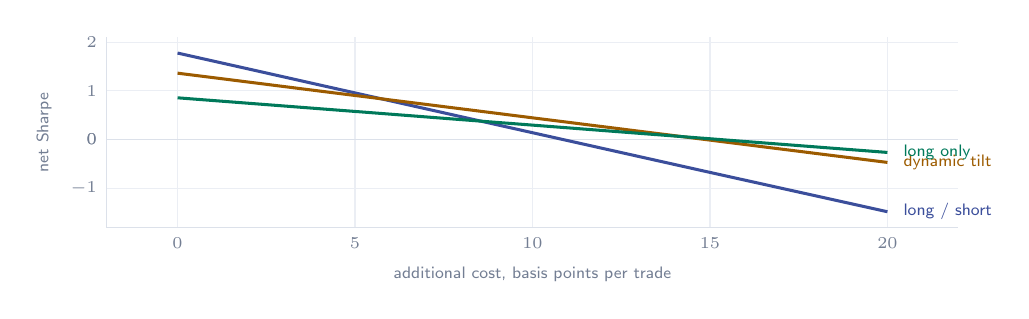
\begin{tikzpicture}\begin{axis}[qrtf,xlabel={additional cost, basis points per trade},ylabel={net Sharpe},xtick={0,5,10,15,20},extra y ticks={0},extra y tick style={grid=major,grid style={hair,line width=0.5pt}},enlarge x limits=0.1,]\addplot[cA,line width=1.1pt,mark=none] coordinates{(0.0000,1.77800) (2.0000,1.45100) (4.0000,1.12300) (6.0000,0.79600) (8.0000,0.46900) (10.0000,0.14200) (15.0000,-0.67300) (20.0000,-1.48100)};\node[anchor=west,font=\sffamily\fontsize{6.4}{8}\selectfont,text=cA,xshift=0.8mm] at (axis cs:20.0000,-1.48100){long / short};\addplot[cD,line width=1.1pt,mark=none] coordinates{(0.0000,1.36500) (2.0000,1.18200) (4.0000,0.99800) (6.0000,0.81500) (8.0000,0.63200) (10.0000,0.44800) (15.0000,-0.01000) (20.0000,-0.46800)};\node[anchor=west,font=\sffamily\fontsize{6.4}{8}\selectfont,text=cD,xshift=0.8mm] at (axis cs:20.0000,-0.46800){dynamic tilt};\addplot[cB,line width=1.1pt,mark=none] coordinates{(0.0000,0.85900) (2.0000,0.74700) (4.0000,0.63500) (6.0000,0.52300) (8.0000,0.41000) (10.0000,0.29800) (15.0000,0.01800) (20.0000,-0.26300)};\node[anchor=west,font=\sffamily\fontsize{6.4}{8}\selectfont,text=cB,xshift=0.8mm] at (axis cs:20.0000,-0.26300){long only};\end{axis}\end{tikzpicture}\end{center}\vskip1mm\figcaption{Sharpe against additional trading cost, in basis points per transaction. The passing configurations stop passing at about 6.8 and 7.8 basis points — less than 2× headroom on a quantity that had not been measured. Horizontal axis: basis points.}\end{column}\end{columns}
\note{The key number: under 2× headroom. That is what made the phase necessary rather than optional.}\end{frame}
\eyebrow{Phase 4b}
\begin{frame}[t]{Three quantities the backtest had not measured \textnormal{\itshape --- continued}}
\begin{columns}[T]\begin{column}{0.475\textwidth}\aside{The first of these decides the outcome. Each additional basis point of trading cost removes roughly 2.1\% a year from the long/short book, because it turns over most of its positions every day.}\end{column}\begin{column}{0.475\textwidth}\end{column}\end{columns}
\end{frame}
\eyebrow{Phase 4c}
\begin{frame}[t]{Phase 4c — measuring all three, and proving nothing else changed}
\vskip1mm\begin{center}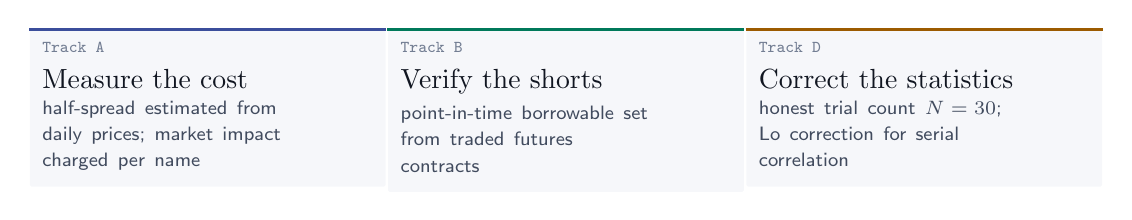
\begin{tikzpicture}[node distance=0mm]
\node[anchor=north west,inner sep=1.6mm,text width=42mm,fill=sunken,rounded corners=0.6pt] (n1) at (0.0mm,0) {{\ttfamily\fontsize{5.6}{7}\selectfont\color{muted}Track A}\\[0.4mm]{\dispfont\fontsize{10}{11}\selectfont\color{ink}Measure the cost}\\[0.8mm]{\sffamily\fontsize{6.6}{8.4}\selectfont\color{ink2}\begin{tabular}{@{}l@{}}half-spread estimated from\\[0.4mm]daily prices; market impact\\[0.4mm]charged per name\end{tabular}}};
\draw[cA,line width=1.1pt] (n1.north west)--(n1.north east);
\node[anchor=north west,inner sep=1.6mm,text width=42mm,fill=sunken,rounded corners=0.6pt] (n3) at (45.5mm,0) {{\ttfamily\fontsize{5.6}{7}\selectfont\color{muted}Track B}\\[0.4mm]{\dispfont\fontsize{10}{11}\selectfont\color{ink}Verify the shorts}\\[0.8mm]{\sffamily\fontsize{6.6}{8.4}\selectfont\color{ink2}\begin{tabular}{@{}l@{}}point-in-time borrowable set\\[0.4mm]from traded futures\\[0.4mm]contracts\end{tabular}}};
\draw[cB,line width=1.1pt] (n3.north west)--(n3.north east);
\node[anchor=north west,inner sep=1.6mm,text width=42mm,fill=sunken,rounded corners=0.6pt] (n5) at (91.0mm,0) {{\ttfamily\fontsize{5.6}{7}\selectfont\color{muted}Track D}\\[0.4mm]{\dispfont\fontsize{10}{11}\selectfont\color{ink}Correct the statistics}\\[0.8mm]{\sffamily\fontsize{6.6}{8.4}\selectfont\color{ink2}\begin{tabular}{@{}l@{}}honest trial count $N=30$;\\[0.4mm]Lo correction for serial\\[0.4mm]correlation\end{tabular}}};
\draw[cD,line width=1.1pt] (n5.north west)--(n5.north east);
\end{tikzpicture}\end{center}\vskip1mm
\note{This slide is the methodological core. If there is one thing to defend, it is that the regression gate ran before any new number was believed.}\end{frame}
\eyebrow{Phase 4c}
\begin{frame}[t]{Phase 4c — measuring all three, and proving nothing else changed \textnormal{\itshape --- continued}}
\begin{columns}[T]\begin{column}{0.475\textwidth}\subhead{The control that makes the comparison valid}
\bodytext{Every addition was written so that it is \str{switched off by default}. With the switches off, the earlier runs were re-executed and had to reproduce their previous output before any new figure was accepted.}
\vskip0.8mm
\bodytext{They reproduced to the last decimal: a maximum difference of \mn{1.1 × $10^{-16}$} across all three Phase 4b configurations, which is the rounding error of the arithmetic itself, and exactly \mn{0.0} on the Phase 3 ledger.}
\vskip0.8mm\end{column}\begin{column}{0.475\textwidth}\subhead{Why that matters}
\bodytext{Rewriting a backtest and getting a different answer leaves two possible explanations: the new measurement, or a mistake introduced while rewriting.}
\vskip0.8mm
\bodytext{Because the old configuration still returns the old numbers exactly, every difference reported from here on is attributable to the cost and eligibility models, and not to the rewrite.}
\vskip0.8mm
\aside{A further rule: a strategy restricted to borrowable shorts is treated as a \emph{different} strategy with its own entry in the trial count, not as a corrected version of the old one. Running both and reporting the better is the error the gate exists to catch.}
\vskip0.8mm\end{column}\end{columns}
{\sffamily\fontsize{6.6}{8.8}\selectfont\color{ink2}\begin{tabular}{lrr}\toprule \textsc{\fontsize{5.8}{7}\selectfont re-run with the new measurements off} & \textsc{\fontsize{5.8}{7}\selectfont columns} & \textsc{\fontsize{5.8}{7}\selectfont largest difference from the published result} \\ \midrule Phase 3, daily, 5-day target & 3 & \mn{0.0} — bit for bit \\ Phase 4b, 500 names, 5-day target & 3 & \mn{1.1 × $10^{-16}$} — floating-point rounding \\ \bottomrule\end{tabular}}
\end{frame}
\eyebrow{Phase 4c}
\begin{frame}[t]{Track A — measuring the spread that had been assumed away}
\begin{center}\setlength{\plotwidth}{124mm}\setlength{\plotheight}{36mm}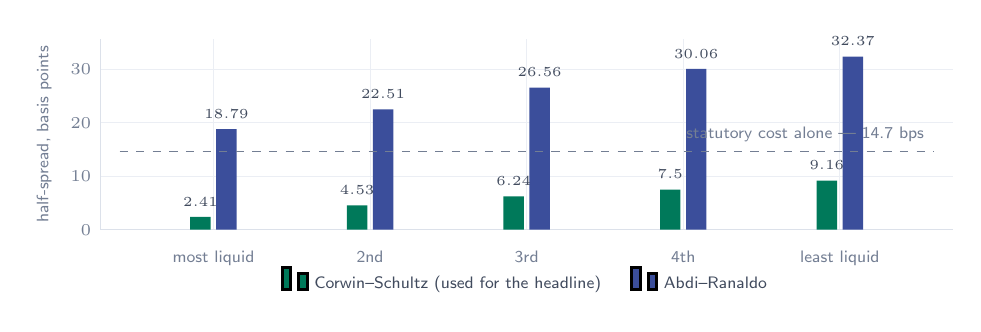
\begin{tikzpicture}\begin{axis}[qrtf,ybar,bar width=2.6mm,xtick={0,1,2,3,4},xticklabels={{most liquid},{2nd},{3rd},{4th},{least liquid}},xtick style={draw=none},enlarge x limits=0.18,ylabel={half-spread, basis points},ymin=0,legend style={at={(0.5,-0.16)},anchor=north,legend columns=-1,/tikz/every even column/.append style={column sep=3mm}},]\addplot[ybar,fill=cB,draw=none,nodes near coords,every node near coord/.append style={font=\ttfamily\fontsize{5.4}{6}\selectfont,color=ink2,/pgf/number format/.cd,fixed,precision=2},] coordinates{(0.0000,2.41000) (1.0000,4.53000) (2.0000,6.24000) (3.0000,7.50000) (4.0000,9.16000)};\addlegendentry{Corwin--Schultz (used for the headline)}\addplot[ybar,fill=cA,draw=none,nodes near coords,every node near coord/.append style={font=\ttfamily\fontsize{5.4}{6}\selectfont,color=ink2,/pgf/number format/.cd,fixed,precision=2},] coordinates{(0.0000,18.79000) (1.0000,22.51000) (2.0000,26.56000) (3.0000,30.06000) (4.0000,32.37000)};\addlegendentry{Abdi--Ranaldo}\draw[muted,dashed,line width=0.5pt](axis cs:-0.6,14.6558)--(axis cs:4.6,14.6558);\node[anchor=south east,font=\sffamily\fontsize{5.8}{7}\selectfont,text=muted] at (axis cs:4.6,14.6558){statutory cost alone --- 14.7 bps};\end{axis}\end{tikzpicture}\end{center}\figcaption{Estimated half-spread by liquidity, both estimators, 500-name universe. From the Phase 4c measurement record (docs/phase4c\_results.md §1).}\vskip2.2mm\begin{columns}[T]\begin{column}{0.475\textwidth}\bodytext{The daily exchange archive records no bid and ask prices, so the spread has to be \emph{estimated} from the open, high, low and close. Two published estimators were used and kept as a range, because they are known to err in opposite directions: Corwin–Schultz reads low at \str{5.97 bps} and Abdi–Ranaldo reads high at \str{26.07 bps}.}\end{column}\begin{column}{0.475\textwidth}\end{column}\end{columns}
\note{Two method points worth mentioning only if asked: between 39\% and 76\% of daily estimates round to zero, so the validation used the mean rather than the median; and the negative-estimate clip is applied once per window, because clipping each observation turns symmetric noise into upward bias.}\end{frame}
\eyebrow{Phase 4c}
\begin{frame}[t]{Track A — measuring the spread that had been assumed away \textnormal{\itshape --- continued}}
\begin{columns}[T]\begin{column}{0.475\textwidth}\bodytext{The strategy grid was run on the \str{lower} estimate deliberately. If the result fails under the generous assumption, the conclusion cannot be attributed to a pessimistic choice of estimator.}\end{column}\begin{column}{0.475\textwidth}\bodytext{Both estimators rise monotonically as stocks become less liquid, which was the condition set in advance for trusting them. Once charged, the real cost of a transaction is about \str{26 bps} against the \str{14.7 bps} of statutory charges — and the long/short Sharpe falls from \str{1.78 to −0.23}.}\end{column}\end{columns}
\end{frame}
\eyebrow{Phase 4c}
\begin{frame}[t]{Track B — most of the short book could not have been borrowed}
\begin{center}\setlength{\plotwidth}{124mm}\setlength{\plotheight}{40mm}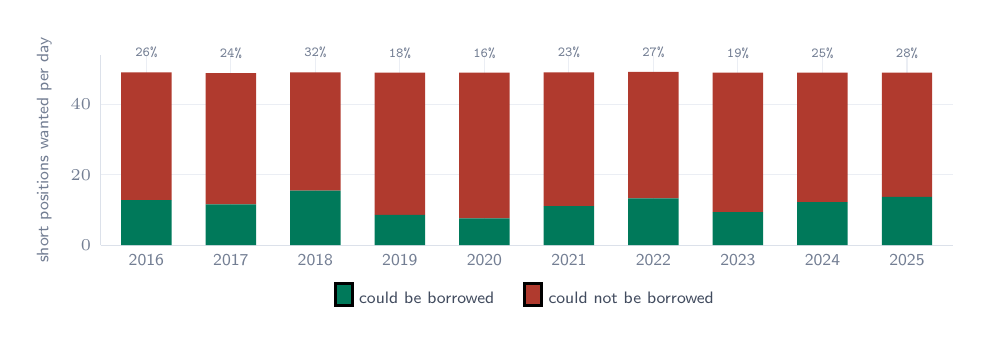
\begin{tikzpicture}\begin{axis}[qrtf,ybar stacked,bar width=6.4mm,xtick={0,1,2,3,4,5,6,7,8,9},xticklabels={{2016},{2017},{2018},{2019},{2020},{2021},{2022},{2023},{2024},{2025}},xtick style={draw=none},enlarge x limits=0.06,ymin=0,ylabel={short positions wanted per day},legend style={at={(0.5,-0.16)},anchor=north,legend columns=-1,/tikz/every even column/.append style={column sep=3mm}},]\addplot[ybar,fill=cB,draw=none] coordinates{(0.0000,12.80000) (1.0000,11.60000) (2.0000,15.50000) (3.0000,8.60000) (4.0000,7.60000) (5.0000,11.10000) (6.0000,13.30000) (7.0000,9.40000) (8.0000,12.20000) (9.0000,13.70000)};\addlegendentry{could be borrowed}\addplot[ybar,fill=cC,draw=none] coordinates{(0.0000,36.30000) (1.0000,37.30000) (2.0000,33.60000) (3.0000,40.40000) (4.0000,41.40000) (5.0000,38.00000) (6.0000,35.90000) (7.0000,39.60000) (8.0000,36.80000) (9.0000,35.30000)};\addlegendentry{could not be borrowed}\node[font=\ttfamily\fontsize{5.4}{6}\selectfont,text=muted,anchor=south,yshift=0.6mm] at (axis cs:0,49.10){26\%};\node[font=\ttfamily\fontsize{5.4}{6}\selectfont,text=muted,anchor=south,yshift=0.6mm] at (axis cs:1,48.90){24\%};\node[font=\ttfamily\fontsize{5.4}{6}\selectfont,text=muted,anchor=south,yshift=0.6mm] at (axis cs:2,49.10){32\%};\node[font=\ttfamily\fontsize{5.4}{6}\selectfont,text=muted,anchor=south,yshift=0.6mm] at (axis cs:3,49.00){18\%};\node[font=\ttfamily\fontsize{5.4}{6}\selectfont,text=muted,anchor=south,yshift=0.6mm] at (axis cs:4,49.00){16\%};\node[font=\ttfamily\fontsize{5.4}{6}\selectfont,text=muted,anchor=south,yshift=0.6mm] at (axis cs:5,49.10){23\%};\node[font=\ttfamily\fontsize{5.4}{6}\selectfont,text=muted,anchor=south,yshift=0.6mm] at (axis cs:6,49.20){27\%};\node[font=\ttfamily\fontsize{5.4}{6}\selectfont,text=muted,anchor=south,yshift=0.6mm] at (axis cs:7,49.00){19\%};\node[font=\ttfamily\fontsize{5.4}{6}\selectfont,text=muted,anchor=south,yshift=0.6mm] at (axis cs:8,49.00){25\%};\node[font=\ttfamily\fontsize{5.4}{6}\selectfont,text=muted,anchor=south,yshift=0.6mm] at (axis cs:9,49.00){28\%};\end{axis}\end{tikzpicture}\end{center}\figcaption{Intended short positions per year, split by whether the name was borrowable. From the Phase 4c feasibility record (docs/phase4c\_results.md §6); the in-universe eligible count independently recomputes to 36\% here.}\vskip2.2mm\begin{columns}[T]\begin{column}{0.475\textwidth}\bodytext{Whether a stock can be sold short was determined from the exchange's derivatives archive: a name is treated as borrowable on a given day only if futures contracts in it actually traded that day. Because it is derived from real trading, it carries no hindsight.}
\vskip0.8mm\end{column}\begin{column}{0.475\textwidth}\bodytext{About a third of the universe qualifies. But the strategy does not want a random third — it wants the \str{50 worst-ranked names}, and those are systematically the ones no lender offers.}\end{column}\end{columns}
\note{This finding voids Phase 4b's two passing cells on its own, independently of cost. Both of them required a book that could not have been held.}\end{frame}
\eyebrow{Phase 4c}
\begin{frame}[t]{Track B — most of the short book could not have been borrowed \textnormal{\itshape --- continued}}
\begin{columns}[T]\begin{column}{0.475\textwidth}\bodytext{Averaged over the sample the strategy intended to short \str{49 names} a day and could have borrowed \str{11}. Coverage never exceeds 32\% in any year. Roughly \str{78\% of the short book was never available}, and because futures eligibility is more generous than actual stock lending, even that is an upper bound.}\end{column}\begin{column}{0.475\textwidth}\bodytext{Restricting the strategy to what it could have borrowed cuts the long/short book's Sharpe \emph{before costs} from \str{4.20 to 1.88}. More than half the raw signal lived in positions that could not have been taken.}\end{column}\end{columns}
\end{frame}
\eyebrow{Phase 4c}
\begin{frame}[t]{Track D — counting the attempts honestly}
\begin{columns}[T]\begin{column}{0.40\textwidth}\bodytext{If thirty strategies are tested, the best of them will look impressive even when none has any skill, simply because it is the maximum of thirty draws. The gate corrects for this by raising the Sharpe a strategy must beat as the number of attempts grows.}
\vskip0.8mm
\bodytext{Phase 4b had used \str{N = 3}. Phase 4c replaced this with a line-by-line tally of every configuration the project had ever run: \str{N = 30}. The bar rises from \str{0.39} to \str{0.98}.}
\vskip0.8mm
\bodytext{A second correction was applied for the fact that overlapping multi-day forecasts make consecutive returns related to one another, which flatters the Sharpe ratio.}\end{column}\begin{column}{0.575\textwidth}\begin{center}\setlength{\plotwidth}{74mm}\setlength{\plotheight}{42mm}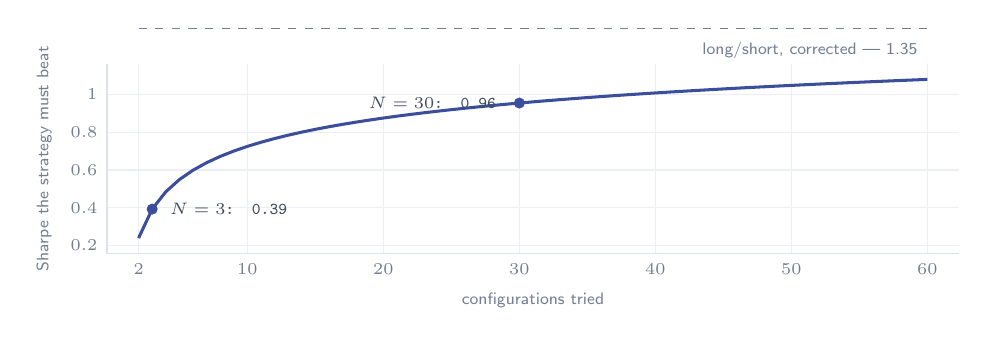
\begin{tikzpicture}\begin{axis}[qrtf,xlabel={configurations tried},ylabel={Sharpe the strategy must beat},xtick={2,10,20,30,40,50,60},enlarge x limits=0.04,]\addplot[cA,line width=1.1pt,mark=none] coordinates{(2.0000,0.23927) (3.0000,0.39260) (4.0000,0.48436) (5.0000,0.54902) (6.0000,0.59853) (7.0000,0.63842) (8.0000,0.67167) (9.0000,0.70011) (10.0000,0.72488) (11.0000,0.74680) (12.0000,0.76641) (13.0000,0.78415) (14.0000,0.80031) (15.0000,0.81515) (16.0000,0.82886) (17.0000,0.84158) (18.0000,0.85345) (19.0000,0.86456) (20.0000,0.87501) (21.0000,0.88486) (22.0000,0.89418) (23.0000,0.90301) (24.0000,0.91141) (25.0000,0.91941) (26.0000,0.92705) (27.0000,0.93435) (28.0000,0.94134) (29.0000,0.94806) (30.0000,0.95451) (31.0000,0.96072) (32.0000,0.96670) (33.0000,0.97247) (34.0000,0.97804) (35.0000,0.98343) (36.0000,0.98864) (37.0000,0.99369) (38.0000,0.99859) (39.0000,1.00334) (40.0000,1.00795) (41.0000,1.01243) (42.0000,1.01680) (43.0000,1.02104) (44.0000,1.02517) (45.0000,1.02920) (46.0000,1.03313) (47.0000,1.03696) (48.0000,1.04070) (49.0000,1.04435) (50.0000,1.04792) (51.0000,1.05141) (52.0000,1.05482) (53.0000,1.05816) (54.0000,1.06143) (55.0000,1.06463) (56.0000,1.06776) (57.0000,1.07084) (58.0000,1.07385) (59.0000,1.07680) (60.0000,1.07970)};\draw[muted,dashed,line width=0.5pt](axis cs:2,1.35)--(axis cs:60,1.35);\node[anchor=north east,font=\sffamily\fontsize{5.8}{7}\selectfont,text=muted] at (axis cs:60,1.33){long/short, corrected --- 1.35};\addplot[only marks,mark=*,mark size=1.4pt,cA] coordinates{(3,0.3926) (30,0.9545)};\node[anchor=west,font=\ttfamily\fontsize{5.6}{7}\selectfont,text=ink2] at (axis cs:3.6,0.3926){$N=3$: 0.39};\node[anchor=east,font=\ttfamily\fontsize{5.6}{7}\selectfont,text=ink2] at (axis cs:29,0.9545){$N=30$: 0.96};\end{axis}\end{tikzpicture}\end{center}\vskip1mm\figcaption{The deflation benchmark as a function of the number of configurations searched, computed with the repository's own estimator at the measured cross-trial dispersion. Horizontal axis: configurations tried.}\end{column}\end{columns}
\note{The methods point, if it comes up: the textbook lag-by-lag correction was implemented first and rejected on measurement — on random data it returned adjustments between 0.99 and 1.18 depending only on the seed, so it was measuring its own noise. The variance-ratio form centres on 1.000 and recovers theory to 0.01.}\end{frame}
\eyebrow{Phase 4c}
\begin{frame}[t]{Track D — counting the attempts honestly \textnormal{\itshape --- continued}}
{\sffamily\fontsize{6.6}{8.8}\selectfont\color{ink2}\begin{tabular}{lrrr}\toprule \textsc{\fontsize{5.8}{7}\selectfont configuration} & \textsc{\fontsize{5.8}{7}\selectfont Sharpe as reported} & \textsc{\fontsize{5.8}{7}\selectfont after both corrections} & \textsc{\fontsize{5.8}{7}\selectfont gate} \\ \midrule long / short & 1.78 & 1.35 & \pillok{0.986} \\ dynamic tilt & 1.37 & 1.20 & \pillok{0.954} \\ long only & 0.86 & 0.77 & \pillno{0.671} \\ \bottomrule\end{tabular}}
\aside{Applied on their own, the statistical corrections do \str{not} overturn Phase 4b — the long/short book still passes at 0.986. The change of verdict comes from the measured costs.}
\end{frame}
\eyebrow{Phase 4c}
\begin{frame}[t]{The committed grid — none of the six passes}
\begin{center}\setlength{\plotwidth}{124mm}\setlength{\plotheight}{35mm}\begin{tikzpicture}\begin{axis}[qrtf,xtick={0,1,2,3,4,5},xticklabels={{long only},{long/short},{dynamic tilt},{long only},{long/short},{dynamic tilt}},xtick style={draw=none},x tick label style={font=\sffamily\fontsize{6.2}{8}\selectfont,color=muted},enlarge x limits=0.06,ylabel={annualized Sharpe ratio},extra y ticks={0},extra y tick style={grid=major,grid style={hair,line width=0.5pt}},]\draw[hair,line width=2.2pt,line cap=round](axis cs:0,1.6596)--(axis cs:0,0.1784);\draw[hair,line width=2.2pt,line cap=round](axis cs:1,1.8821)--(axis cs:1,-0.9866);\draw[hair,line width=2.2pt,line cap=round](axis cs:2,2.0145)--(axis cs:2,-0.0492);\draw[hair,line width=2.2pt,line cap=round](axis cs:3,1.1199)--(axis cs:3,0.2975);\draw[hair,line width=2.2pt,line cap=round](axis cs:4,0.9579)--(axis cs:4,-0.5666);\draw[hair,line width=2.2pt,line cap=round](axis cs:5,1.3075)--(axis cs:5,0.2119);\addplot[only marks,mark=*,mark size=1.5pt,cA] coordinates{(0.0000,1.65957) (1.0000,1.88212) (2.0000,2.01445) (3.0000,1.11990) (4.0000,0.95785) (5.0000,1.30752)};\addplot[only marks,mark=*,mark size=1.5pt,cB] coordinates{(0.0000,0.17841) (3.0000,0.29745) (5.0000,0.21192)};\addplot[only marks,mark=*,mark size=1.5pt,cC] coordinates{(1.0000,-0.98657) (2.0000,-0.04924) (4.0000,-0.56660)};\node[anchor=west,font=\ttfamily\fontsize{5.4}{6}\selectfont,text=ink2,xshift=1mm,yshift=0.0mm] at (axis cs:0,1.6596){1.66};\node[anchor=west,font=\ttfamily\fontsize{5.4}{6}\selectfont,text=cB,xshift=1mm,yshift=0.0mm] at (axis cs:0,0.1784){0.18};\node[anchor=west,font=\ttfamily\fontsize{5.4}{6}\selectfont,text=ink2,xshift=1mm,yshift=0.0mm] at (axis cs:1,1.8821){1.88};\node[anchor=west,font=\ttfamily\fontsize{5.4}{6}\selectfont,text=cC,xshift=1mm,yshift=0.0mm] at (axis cs:1,-0.9866){−0.99};\node[anchor=west,font=\ttfamily\fontsize{5.4}{6}\selectfont,text=ink2,xshift=1mm,yshift=0.0mm] at (axis cs:2,2.0145){2.01};\node[anchor=west,font=\ttfamily\fontsize{5.4}{6}\selectfont,text=cC,xshift=1mm,yshift=0.0mm] at (axis cs:2,-0.0492){−0.05};\node[anchor=west,font=\ttfamily\fontsize{5.4}{6}\selectfont,text=ink2,xshift=1mm,yshift=0.0mm] at (axis cs:3,1.1199){1.12};\node[anchor=west,font=\ttfamily\fontsize{5.4}{6}\selectfont,text=cB,xshift=1mm,yshift=0.0mm] at (axis cs:3,0.2975){0.30};\node[anchor=west,font=\ttfamily\fontsize{5.4}{6}\selectfont,text=ink2,xshift=1mm,yshift=0.0mm] at (axis cs:4,0.9579){0.96};\node[anchor=west,font=\ttfamily\fontsize{5.4}{6}\selectfont,text=cC,xshift=1mm,yshift=0.0mm] at (axis cs:4,-0.5666){−0.57};\node[anchor=west,font=\ttfamily\fontsize{5.4}{6}\selectfont,text=ink2,xshift=1mm,yshift=0.0mm] at (axis cs:5,1.3075){1.31};\node[anchor=west,font=\ttfamily\fontsize{5.4}{6}\selectfont,text=cB,xshift=1mm,yshift=0.0mm] at (axis cs:5,0.2119){0.21};\node[font=\ttfamily\fontsize{5.2}{6}\selectfont,text=muted,anchor=north,yshift=-3.4mm] at (axis cs:0,\pgfkeysvalueof{/pgfplots/ymin}){DSR 0.007};\node[font=\ttfamily\fontsize{5.2}{6}\selectfont,text=muted,anchor=north,yshift=-3.4mm] at (axis cs:1,\pgfkeysvalueof{/pgfplots/ymin}){DSR 0.000};\node[font=\ttfamily\fontsize{5.2}{6}\selectfont,text=muted,anchor=north,yshift=-3.4mm] at (axis cs:2,\pgfkeysvalueof{/pgfplots/ymin}){DSR 0.001};\node[font=\ttfamily\fontsize{5.2}{6}\selectfont,text=muted,anchor=north,yshift=-3.4mm] at (axis cs:3,\pgfkeysvalueof{/pgfplots/ymin}){DSR 0.017};\node[font=\ttfamily\fontsize{5.2}{6}\selectfont,text=muted,anchor=north,yshift=-3.4mm] at (axis cs:4,\pgfkeysvalueof{/pgfplots/ymin}){DSR 0.000};\node[font=\ttfamily\fontsize{5.2}{6}\selectfont,text=muted,anchor=north,yshift=-3.4mm] at (axis cs:5,\pgfkeysvalueof{/pgfplots/ymin}){DSR 0.009};\node[font=\sffamily\fontsize{6.2}{8}\selectfont,text=muted,anchor=north,yshift=-6.6mm] at (axis cs:1.0,\pgfkeysvalueof{/pgfplots/ymin}){5-day forecast};\node[font=\sffamily\fontsize{6.2}{8}\selectfont,text=muted,anchor=north,yshift=-6.6mm] at (axis cs:4.0,\pgfkeysvalueof{/pgfplots/ymin}){21-day forecast};\end{axis}\end{tikzpicture}\end{center}\figcaption{Sharpe before and after measured costs for each committed configuration, with its credibility score. Computed from the Phase 4c ledger and gate output.}\vskip2.2mm\begin{columns}[T]\begin{column}{0.475\textwidth}\bodytext{Six configurations were fixed in writing \emph{before} the run: three trading styles, each with a five-day and a twenty-one-day forecast horizon. Fixing them in advance is what stops the search from continuing until something works.}
\vskip0.8mm\end{column}\begin{column}{0.475\textwidth}\bodytext{All six fail. The best reaches a credibility score of \str{0.017} against a threshold of \str{0.95} — under 2\% of the confidence required, not a near miss. For every one of the six, the minimum track record needed to reach credibility is \str{undefined}: none clears the bar at any length of history, so collecting more data would not change the answer.}\end{column}\end{columns}
\note{Every gross value is comfortably positive and every net value is at or below 0.3. The line length is the cost of harvesting the signal.}\end{frame}
\eyebrow{Phase 4c}
\begin{frame}[t]{The committed grid — none of the six passes \textnormal{\itshape --- continued}}
\begin{columns}[T]\begin{column}{0.475\textwidth}\bodytext{The slower forecast horizon did what it was intended to do — turnover fell from \str{0.45 to 0.24} of the book per day and the net Sharpe rose from \str{0.18 to 0.30}. It was the one remaining lever with room in it, and it moved the result by 0.12 against a gate that needed far more.}\end{column}\begin{column}{0.475\textwidth}\end{column}\end{columns}
\end{frame}
\eyebrow{Findings}
\begin{frame}[t]{What each correction was worth}
\begin{center}\setlength{\plotwidth}{124mm}\setlength{\plotheight}{40mm}\begin{tikzpicture}\begin{axis}[qrtf,ybar,xtick={0,1,2,3},xticklabels={{\begin{tabular}{@{}c@{}}as reported\\in Phase 4b\end{tabular}},{\begin{tabular}{@{}c@{}}honest trial count\\and serial correlation\end{tabular}},{\begin{tabular}{@{}c@{}}measured spread\\and market impact\end{tabular}},{\begin{tabular}{@{}c@{}}short book restricted\\to what could be borrowed\end{tabular}}},xtick style={draw=none},enlarge x limits=0.14,x tick label style={font=\sffamily\fontsize{6.4}{8}\selectfont,color=ink2},ylabel={annualized Sharpe ratio},extra y ticks={0},extra y tick style={grid=major,grid style={hair,line width=0.5pt}}]\addplot[ybar,bar width=13mm,fill=cA,draw=none] coordinates{(0.0000,1.78000) (1.0000,1.35000)};\addplot[ybar,bar width=13mm,fill=cC,draw=none] coordinates{(2.0000,-0.23000) (3.0000,-0.99000)};\node[font=\ttfamily\fontsize{6.4}{8}\selectfont,text=ink2,anchor=south,yshift=0.8mm] at (axis cs:0,1.7800){1.78};\node[font=\sffamily\fontsize{5.8}{7}\selectfont,text=cB,anchor=north,yshift=-7.6mm] at (axis cs:0,\pgfkeysvalueof{/pgfplots/ymin}){\MakeUppercase{clears the gate}};\node[font=\ttfamily\fontsize{6.4}{8}\selectfont,text=ink2,anchor=south,yshift=0.8mm] at (axis cs:1,1.3500){1.35};\draw[muted,dashed,line width=0.4pt](axis cs:0.24,1.7800)--(axis cs:0.76,1.7800);\node[font=\ttfamily\fontsize{5.6}{7}\selectfont,text=muted,anchor=south,yshift=0.4mm] at (axis cs:0.50,1.7800){−0.43};\node[font=\sffamily\fontsize{5.8}{7}\selectfont,text=cB,anchor=north,yshift=-7.6mm] at (axis cs:1,\pgfkeysvalueof{/pgfplots/ymin}){\MakeUppercase{clears the gate}};\node[font=\ttfamily\fontsize{6.4}{8}\selectfont,text=ink2,anchor=north,yshift=-0.8mm] at (axis cs:2,-0.2300){−0.23};\draw[muted,dashed,line width=0.4pt](axis cs:1.24,1.3500)--(axis cs:1.76,1.3500);\node[font=\ttfamily\fontsize{5.6}{7}\selectfont,text=muted,anchor=south,yshift=0.4mm] at (axis cs:1.50,1.3500){−1.58};\node[font=\sffamily\fontsize{5.8}{7}\selectfont,text=cC,anchor=north,yshift=-7.6mm] at (axis cs:2,\pgfkeysvalueof{/pgfplots/ymin}){\MakeUppercase{fails}};\node[font=\ttfamily\fontsize{6.4}{8}\selectfont,text=ink2,anchor=north,yshift=-0.8mm] at (axis cs:3,-0.9900){−0.99};\draw[muted,dashed,line width=0.4pt](axis cs:2.24,-0.2300)--(axis cs:2.76,-0.2300);\node[font=\ttfamily\fontsize{5.6}{7}\selectfont,text=muted,anchor=south,yshift=0.4mm] at (axis cs:2.50,-0.2300){−0.76};\node[font=\sffamily\fontsize{5.8}{7}\selectfont,text=cC,anchor=north,yshift=-7.6mm] at (axis cs:3,\pgfkeysvalueof{/pgfplots/ymin}){\MakeUppercase{fails}};\end{axis}\end{tikzpicture}\end{center}\figcaption{The long/short configuration, Phase 4b to Phase 4c, one correction at a time. Vertical axis: annualized Sharpe ratio.}
\note{Close here. The statistical corrections, which were expected to be decisive, were the mildest of the three; the measured cost of trading was what settled it.}\end{frame}
\eyebrow{Findings}
\begin{frame}[t]{Findings}
\begin{center}\setlength{\plotwidth}{124mm}\setlength{\plotheight}{23mm}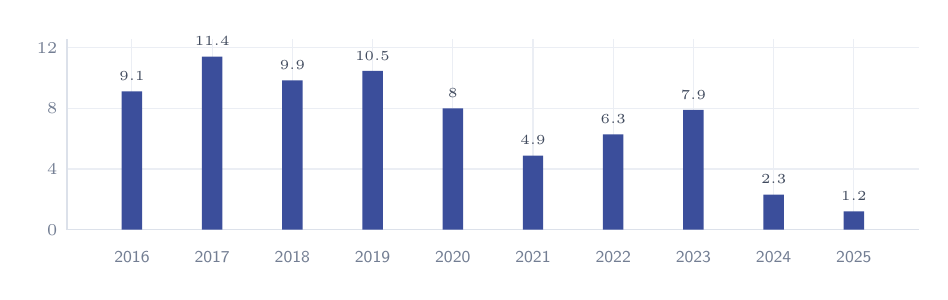
\begin{tikzpicture}\begin{axis}[qrtf,ybar,bar width=2.6mm,xtick={0,1,2,3,4,5,6,7,8,9},xticklabels={{2016},{2017},{2018},{2019},{2020},{2021},{2022},{2023},{2024},{2025}},xtick style={draw=none},enlarge x limits=0.09,ylabel={},ymin=0,ytick={0,4,8,12},legend style={draw=none,fill=none},legend to name=none,]\addplot[ybar,fill=cA,draw=none,nodes near coords,every node near coord/.append style={font=\ttfamily\fontsize{5.4}{6}\selectfont,color=ink2,/pgf/number format/.cd,fixed,precision=1},] coordinates{(0.0000,9.12000) (1.0000,11.42000) (2.0000,9.85000) (3.0000,10.48000) (4.0000,8.00000) (5.0000,4.89000) (6.0000,6.28000) (7.0000,7.91000) (8.0000,2.31000) (9.0000,1.21000)};\addlegendentry{significance of the ranking}\end{axis}\end{tikzpicture}\end{center}\figcaption{Significance of the daily ranking by year, from the Phase 4c diagnostics. A value near 2 is the conventional threshold.}\vskip2mm\begin{columns}[T]\begin{column}{0.475\textwidth}\subhead{The signal is real, and it is not a small-stock illusion}
\bodytext{Skill is flat across the liquidity spectrum — an information coefficient of 0.041 in the most traded fifth of the universe and 0.048 in the least. The leading suspicion, that the edge was an artefact of thinly traded names, is ruled out. The strategy fails because a genuine 0.04 does not cover 26 basis points a side while replacing a quarter to three quarters of the book every day.}
\vskip0.8mm\end{column}\begin{column}{0.475\textwidth}\subhead{The signal is fading}
\bodytext{Its statistical significance falls from about 10 in 2016–2019 to \str{1.21} in 2025, at which point it is indistinguishable from zero.}
\vskip0.8mm\end{column}\end{columns}
\end{frame}
\eyebrow{Findings}
\begin{frame}[t]{Findings}
\begin{columns}[T]\begin{column}{0.475\textwidth}\subhead{The breadth argument is settled, negatively}
\bodytext{Widening the universe from 68 names to 500 produced the predicted improvement before costs. It also raised turnover from 0.32 to 0.45 of the book per day and extended the strategy into stocks with wider spreads. Breadth bought signal and cost together.}
\vskip0.8mm\end{column}\begin{column}{0.475\textwidth}\subhead{What this does not rule out}
\bodytext{A portfolio construction that treats cost as part of the objective rather than a charge applied afterwards; and neutralizing market and sector exposure, deliberately excluded here because it adds a degree of freedom that requires its own committed prior and its own trial count.}
\vskip0.8mm
\aside{Each correction was applied to every configuration alike and regardless of whether it improved the result. That is the basis on which these figures are reported.}
\vskip0.8mm\end{column}\end{columns}
\end{frame}

\end{document}
